\documentclass[11pt,letterpaper]{article}

\newenvironment{proof}{\noindent{\bf Proof:}}{\qed\bigskip}

\newtheorem{theorem}{Theorem}
\newtheorem{corollary}{Corollary}
\newtheorem{lemma}{Lemma} 
\newtheorem{claim}{Claim}
\newtheorem{fact}{Fact}
\newtheorem{definition}{Definition}
\newtheorem{assumption}{Assumption}
\newtheorem{observation}{Observation}
\newtheorem{example}{Example}
\newcommand{\qed}{\rule{7pt}{7pt}}

\newcommand{\solution}[4]{
\thispagestyle{plain} 
\newpage
\setcounter{page}{1}
\noindent
\begin{center}
\framebox{ \vbox{
\vspace{4mm}
\vspace{0.2in} 
{\centering \large\mbox{#3}}\\
\vspace{0.1in}
{#1 \hfill {Date: #2}}
}}
\end{center}
\markright{#1}
}

\newenvironment{algorithm}
{\begin{center}
\begin{tabular}{|l|}
\hline
\begin{minipage}{1in}
\begin{tabbing}
\quad\=\qquad\=\qquad\=\qquad\=\qquad\=\qquad\=\qquad\=\kill}
{\end{tabbing}
\end{minipage} \\
\hline
\end{tabular}
\end{center}}

\def\Comment#1{\textsf{\textsl{$\langle\!\langle$#1\/$\rangle\!\rangle$}}}



\usepackage{graphicx, amssymb, amsmath, listings, float, mathtools}
\usepackage{color, url}
\usepackage{romannum}
\usepackage{subcaption}
\usepackage{mwe}
\lstset{language = Python}
\lstset{breaklines}
\lstset{extendedchars=false}
 
\definecolor{codegreen}{rgb}{0,0.6,0}
\definecolor{codegray}{rgb}{0.5,0.5,0.5}
\definecolor{codepurple}{rgb}{0.58,0,0.82}
\definecolor{backcolour}{rgb}{0.95,0.95,0.92}
 
\lstdefinestyle{mystyle}{
    backgroundcolor=\color{backcolour},   
    commentstyle=\color{codegreen},
    keywordstyle=\color{magenta},
    numberstyle=\tiny\color{codegray},
    stringstyle=\color{codepurple},
    basicstyle=\footnotesize,
    breakatwhitespace=false,         
    breaklines=true,                 
    captionpos=b,                    
    keepspaces=true,                 
    numbers=left,                    
    numbersep=5pt,                  
    showspaces=false,                
    showstringspaces=false,
    showtabs=false,                  
    tabsize=2
}
 
\lstset{style=mystyle}

\oddsidemargin 0in
\evensidemargin 0in
\textwidth 6.5in
\topmargin -0.6in
\textheight 9.0in
\pagenumbering{arabic}

\begin{document}
% -----------------------------------------------------------------------------
\solution{\large Jifu Zhao}{\large 12/15/2016}{\bf \Large IE 529 \hspace{0.5cm} 
		Fall 2016 \hspace{0.5cm} Computational Assignment 2}

% -----------------------------------------------------------------------------
\section{\Large Clustering Result Comparison}

In this part, we have implemented 5 different algorithms for clustering problems: Lloyd's (K-Means) algorithm, Greedy K-Centers algorithm, Single-Swap for K-Centers algorithm, Spectral Clustering and Expectation Maximizaiton algorithm. Since all algorithm have some kind of randomness, to get the best solution that is as close to the global optimum as possiblem, in each algorithm, we change the random state of each algorithm for each run by using Python Numpy function: 
    $$np.random.seed()$$
In this way, for each run, we have different initializations. To find the best solution, we run each algorithm for $50$ times and keep recording the lowest cost. Using the result that corresponds to the lowest cost as the final result.  The details are shown below.

\begin{description}
% -----------------------------------------------------------------------------
\item[(\Romannum{1}).] Lloyd's (K-Means)Algorithm

\begin{description}
\item{1.} In this part, with the Lloyd's algorithm for k-means clustering, we choose the best distortion D as the the objection function. The change of D versus cluster number K is shown in Fig. \ref{fig:k-means-loss}, where the result for clustering.txt is shown in Fig. \ref{fig:1a} and the result for bigClusteringData.txt is show in Fig. \ref{fig:1b}.

%  -----------------------------------------------------------------------------
\begin{figure}[H]
\centering
\centering
        \begin{subfigure}[b]{0.49\textwidth}
            \centering
            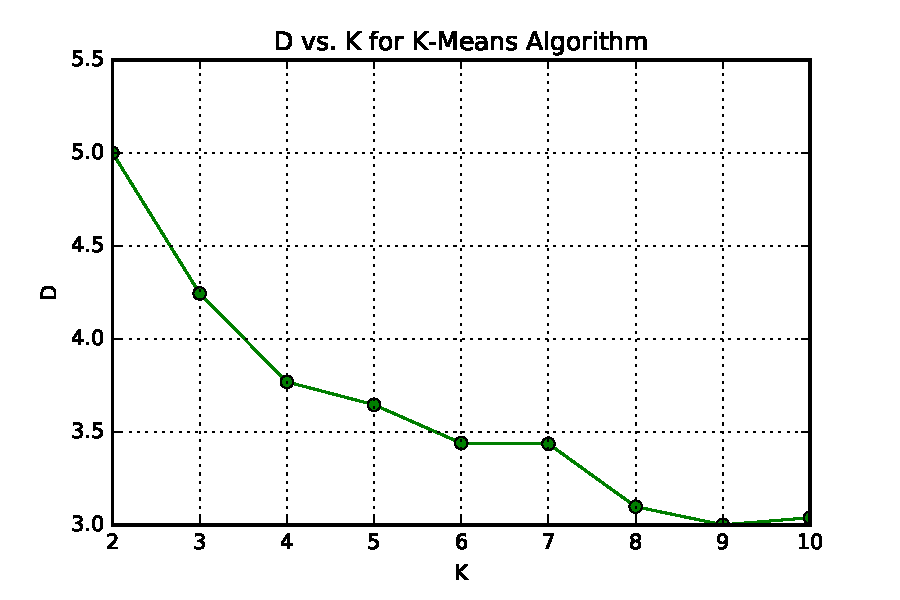
\includegraphics[width=\textwidth]{./figures/loss_clustering_kMeans.pdf}
            \caption{clustering.txt}\label{fig:1a}
        \end{subfigure}
        \hfill
        \begin{subfigure}[b]{0.49\textwidth}  
            \centering 
            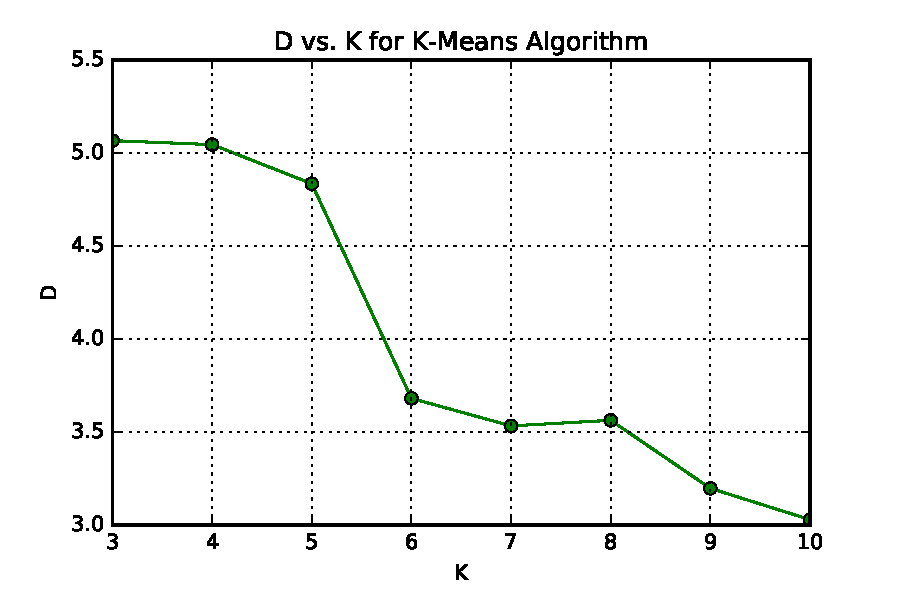
\includegraphics[width=\textwidth]{./figures/loss_bigClustering_kMeans.pdf}
            \caption{bigClusteringData.txt}\label{fig:1b}
        \end{subfigure}
\caption{Change of Distoration versus Cluster Number K for K-Means Algorithm}
\label{fig:k-means-loss} 
\end{figure}

\item{2.} The scatter plot of the clustering result for clustering.txt is shown in Fig. \ref{fig:kmean_clustering} and the scatter plot of the clustering result for bigClusteringData.txt is shown in Fig. \ref{fig:kmean_bigCustering}. The cluster centroids are clearly marked and different clusters are denoted by different colors. \\

%  -----------------------------------------------------------------------------
\begin{figure}[!h]
        \centering
        \begin{subfigure}[b]{0.475\textwidth}
            \centering
            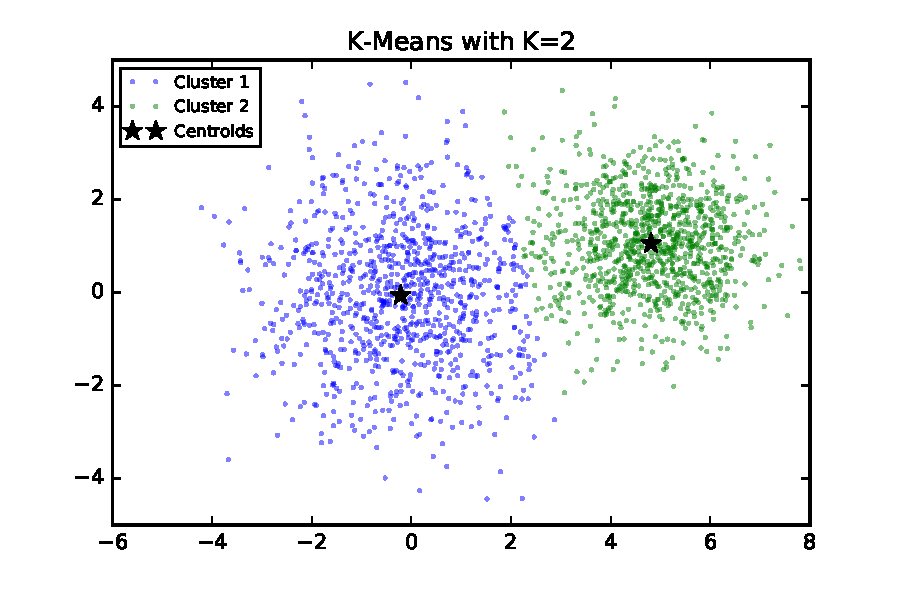
\includegraphics[width=\textwidth]{./figures/clustering_kMeans_2.pdf}
        \end{subfigure}
        \hfill
        \begin{subfigure}[b]{0.475\textwidth}  
            \centering 
            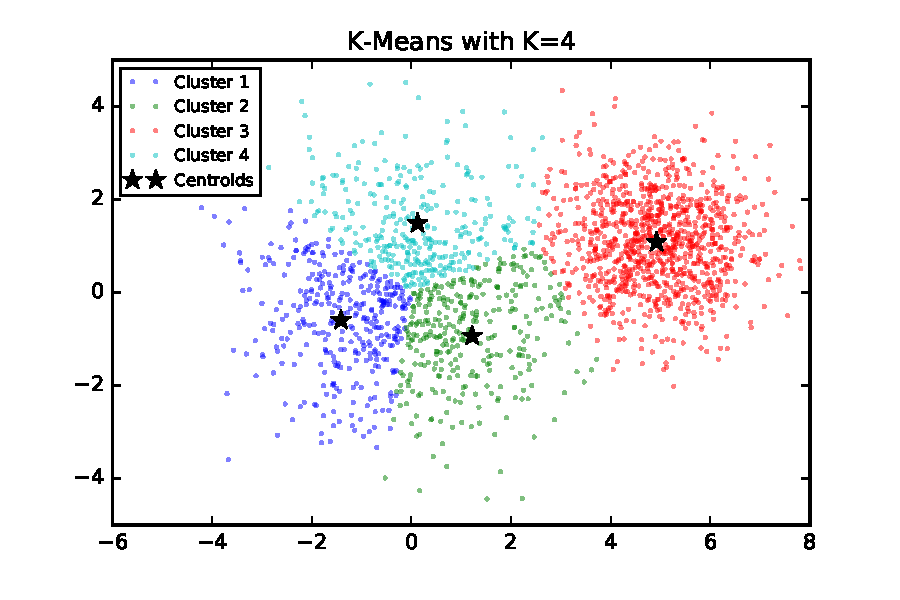
\includegraphics[width=\textwidth]{./figures/clustering_kMeans_4.pdf}
        \end{subfigure}        
        \caption{Clustering Result for clustering.txt with K-Means Algorithm}
        \label{fig:kmean_clustering}
\end{figure}

\vspace{2in}
%  -----------------------------------------------------------------------------
\begin{figure}[!h]
        \centering
        \begin{subfigure}[b]{0.475\textwidth}
            \centering
            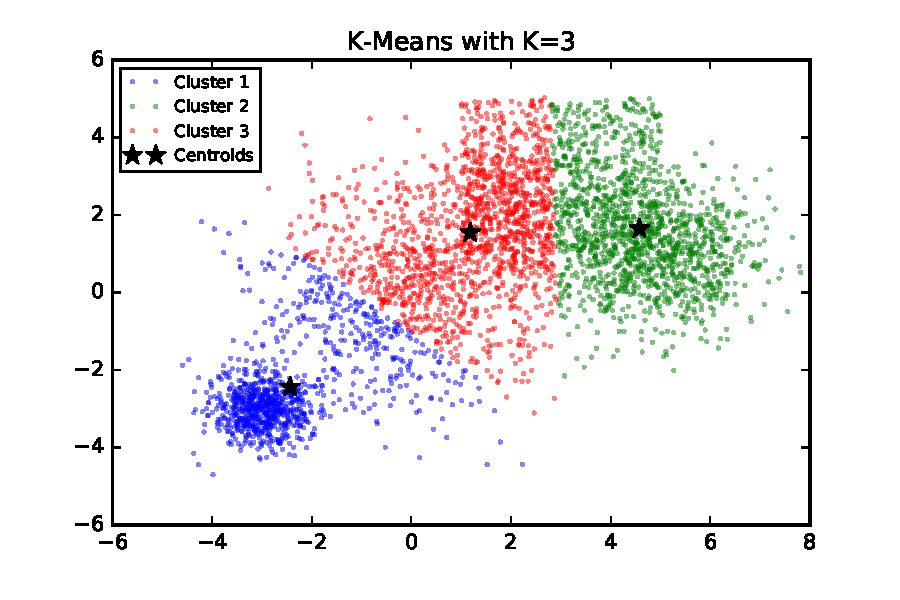
\includegraphics[width=\textwidth]{./figures/bigClustering_kMeans_3.pdf}
        \end{subfigure}
        \hfill  
        \begin{subfigure}[b]{0.475\textwidth}  
            \centering 
            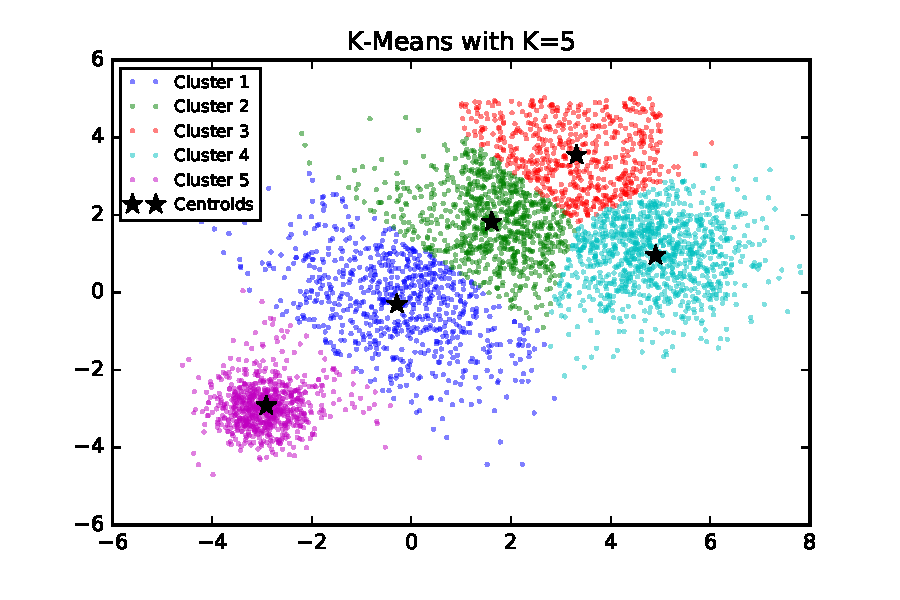
\includegraphics[width=\textwidth]{./figures/bigClustering_kMeans_5.pdf}
        \end{subfigure}
        \begin{subfigure}[b]{0.475\textwidth}   
            \centering 
            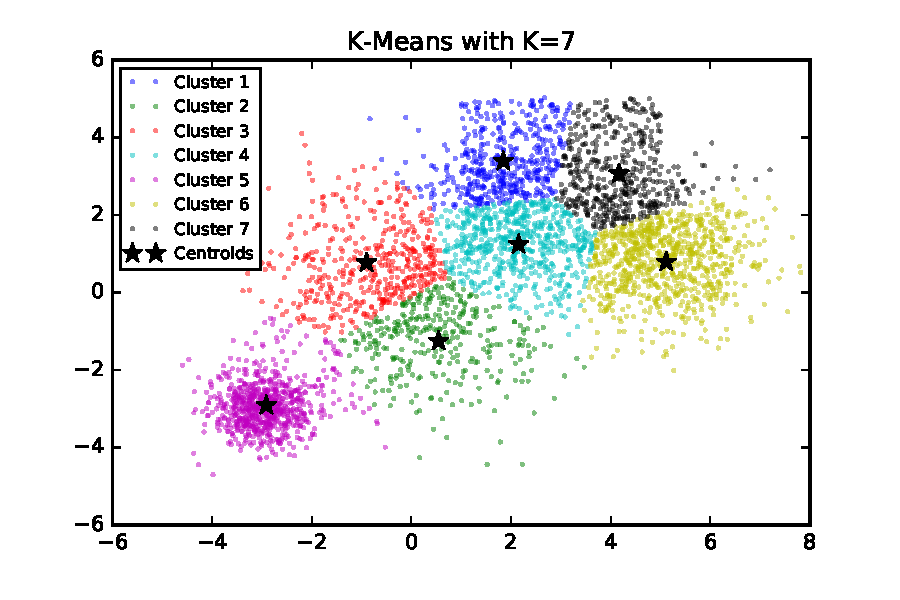
\includegraphics[width=\textwidth]{./figures/bigClustering_kMeans_7.pdf}
        \end{subfigure}
        \hfill
        \begin{subfigure}[b]{0.475\textwidth}   
            \centering 
            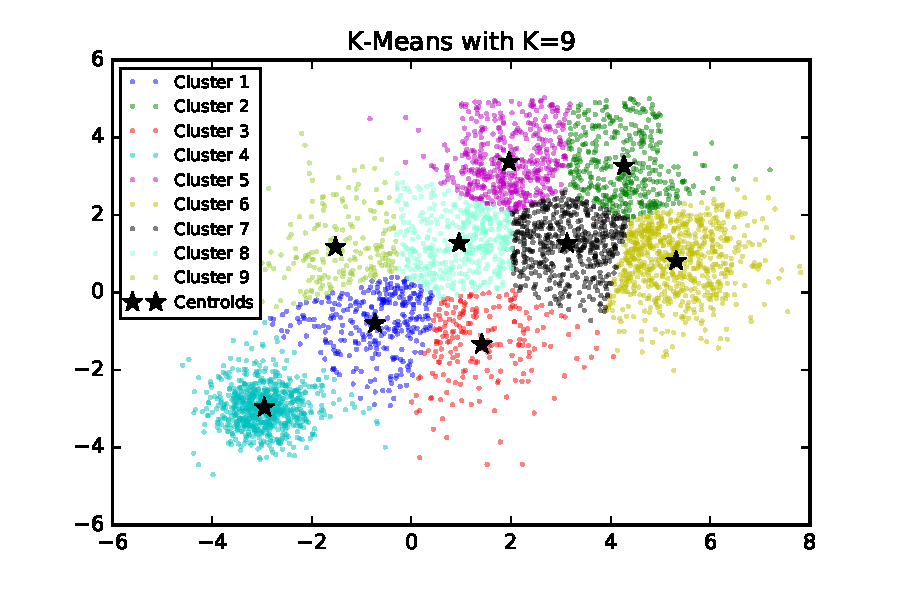
\includegraphics[width=\textwidth]{./figures/bigClustering_kMeans_9.pdf}
        \end{subfigure}        
        
        \caption{Clustering Result for bigClusteringData.txt with K-Means Algorithm}
        \label{fig:kmean_bigCustering}
\end{figure}

\newpage
\item{3.} The Python code used for K-Means Algorithm is shown in Listing 1.

% -----------------------------------------------------------------------------
\begin{lstlisting}[language=Python, caption={K-Means Algorithm Python Code}]
import numpy as np
import time

def kMeans(X, K, tol=0.00001, random_state=None, verbose=True):
    """ function to implement the Lloyd's algorithm for k-means problem """
    np.random.seed(random_state)
    t0 = time.time()

    N, d = X.shape  # number of observations and dimensions
    index = np.random.choice(range(N), size=K, replace=False)
    Y = X[index, :]  # initial k centers
    C = np.zeros(N)
    D = 100
    count = 0
    diff = 100  # difference between D1 and D0

    while diff >= tol:
        D0 = D
        for i in range(N):
            # assign centers to ith data
            C[i] = np.argmin(np.sum((Y - X[i, :]) ** 2, axis=1))

        D = 0
        # re-compute the new centers
        for j in range(K):
            Y[j, :] = np.mean(X[C == j, :], axis=0)

        # compute the loss
        loss = np.zeros((N, K))
        for i in range(K):
            loss[:, i] = np.sqrt(np.sum((X - Y[i, :])**2, axis=1))
        D = np.max(np.min(loss, axis=1))
        diff = abs(D - D0)
        count += 1

    if verbose is True:
        t = np.round(time.time() - t0, 4)
        print('K-Means finished in ' + str(t) + 's, ' + str(count) + ' iters')

    return Y, C, D
\end{lstlisting}

\item{4.} Convergence analysis.

In Lloyd's algorithm, we choose $D = \underset{x_i \in X}{\max}( \underset{c_j \in Q}{\min}{||x_i - c_j||_2})$ as the cost, the stop criterion is: $|D^{p+1} - D^{p}| < tol$, where tol is user-defined. A comparison of cost for clustering.txt and bigClusteringData.txt with different tols are shown in Table \ref{table:tol}.

\begin{table}[H]
	\centering
	\caption{Convergence with different tols for Lloyd's Algorithm}
	\label{table:tol}	
	\begin{tabular}{ c | c | c | c | c | c | c | c | c | c}
		\hline \hline
		Data / tol   & 1E-7    & 1E-6    & 1E-5     & 1E-4    & 1E-3    & 1E-2    & 1E-1    & 1    & 10 \\[0.1cm]
		\hline
	clustering	       & 4.5434 & 4.3220    & 4.5206    & 4.8404    & 4.5841    & 4.9737 & 4.4175 & 5.0615 & 4.9204 \\[0.1cm]
bigClusteringData & 5.0665 & 5.0665    & 5.1257    & 5.0665    & 5.0665    & 5.0569 & 4.8251 & 5.0097 & 5.4848 \\[0.1cm]
		\hline	
	\end{tabular}
\end{table}
Note: here we choose $K = 3$.\\

In Table \ref{table:tol}, we only run the code one time, the solution is not optimal. But as we increase the tol from $1E-7$ to $10$, the final cost D tends to increase, which is consistent with our theoretical analysis.\\

\item{5.} Different Initialization Comparison.

In Lloyd's algorithm, we run 50 times with different initialization and fix $$tol = 1E-5$$
the best result of D is shown in Table \ref{table:best_kmeans}.

\begin{table}[H]
	\centering
	\caption{Best Result (D) for Lloyd's Algorithm}
	\label{table:best_kmeans}	
	\begin{tabular}{ c | c | c | c | c | c | c | c | c | c}
		\hline \hline
		Data / K      &  2        &     3    & 4    & 5     & 6    & 7    & 8   & 9    & 10 \\[0.1cm]
		\hline
	clustering	        & 5.0008 & 4.2447 & 3.8771 & 3.6497 & 3.5388 & 3.3601 & 3.2111 & 3.0413 & 2.9365 \\[0.1cm]
bigClusteringData & N.A.    & 5.0665 & 5.0450 & 4.8319 & 3.6807 & 3.5872 & 3.5485 & 3.0802 & 3.0375 \\[0.1cm]
		\hline	
	\end{tabular}
\end{table}

\item{6.} Cluster Index Comparison.

In Lloyd's algorithm, the cluster index set C (first 20) for the best result is shown in Table \ref{table:index_kmeans_clustering} and Table \ref{table:index_kmeans_bigClustering}.

\begin{table}[H]
	\centering
	\caption{Index (first 20) for Lloyd's Algorithm (clustering.txt)}
	\label{table:index_kmeans_clustering}	
	\begin{tabular}{ c | c }
		\hline \hline
		K        &    Index  \\[0.1cm]
		\hline
		2     &  0  0  0  0  0  0  0  0  0  0  0  0  0  0  0  0  0  0  0  0 \\[0.1cm]
		3     &  0  0  2  0  2  2  2  0  2  0  2  0  2  2  0  2  2  0  0  2 \\[0.1cm]
		4     &  2  3  3  3  1  1  1  2  1  2  1  2  1  1  2  1  1  2  3  1 \\[0.1cm]
		5     &  0  3  3  3  1  1  1  0  1  0  1  0  1  4  0  1  1  0  3  1 \\[0.1cm]
		6     &  4  4  3  4  3  5  5  4  5  5  5  2  5  5  4  5  5  2  4  5 \\[0.1cm]
		7     &  6  6  5  2  5  6  6  2  3  6  3  6  3  3  2  3  6  0  6  6 \\[0.1cm]
		8     &  4  6  6  2  3  5  5  4  5  5  5  4  3  5  2  5  3  4  6  5 \\[0.1cm]
		9     &  8  8  0  8  1  8  8  7  4  8  8  8  1  4  7  1  1  3  8  4 \\[0.1cm]
		10   &  7  7  3  7  2  0  7  5  0  7  0  7  2  1  4  0  0  5  7  0 \\[0.1cm]
		\hline	
	\end{tabular}
\end{table}

\begin{table}[H]
	\centering
	\caption{Index (first 20) for Lloyd's Algorithm (bigClusteringData.txt)}
	\label{table:index_kmeans_bigClustering}	
	\begin{tabular}{ c | c }
		\hline \hline
		K    & Index \\[0.1cm]
		\hline
		3     &  2  0  1  0  0  1  0  1  0  1  0  1  2  2  0  0  2  0  0  0 \\[0.1cm]
		4     &  0  3  2  1  1  2  1  2  1  2  3  1  0  0  1  1  3  3  3  1 \\[0.1cm]
		5     &  3  2  4  2  2  4  2  4  2  4  2  1  3  3  2  1  0  2  0  1 \\[0.1cm]
		6     &  3  5  1  5  2  1  4  1  5  1  5  2  3  3  5  4  0  5  0  4 \\[0.1cm]
		7     &  5  0  3  0  4  3  0  3  0  3  0  4  6  5  0  2  6  0  1  4 \\[0.1cm]
		8     &  7  0  4  2  2  4  6  4  0  4  0  1  5  7  0  6  5  0  3  6 \\[0.1cm]
		9     &  6  0  1  3  3  1  4  1  3  1  0  8  2  6  3  4  2  0  5  3 \\[0.1cm]
		10   &  6  8  0  8  8  0  1  0  8  0  8  9  2  6  8  1  4  8  3  7 \\[0.1cm]
		\hline	
	\end{tabular}
\end{table}

\end{description}

% -----------------------------------------------------------------------------
\item[(\Romannum{2}).] Greedy K-Centers Algorithm

\begin{description}
\item{1.} In this part, with the Greedy K-Centers Algorithm, we choose 
$$D = \underset{x_i \in X}{\max}( \underset{c_j \in Q}{\min}{||x_i - c_j||_2})$$
as the the objection function. The change of D versus cluster number K is shown in Fig. \ref{fig:k-centers-loss}, where the result for clustering.txt is shown in Fig. \ref{fig:4a} and the result for bigClusteringData.txt is show in Fig. \ref{fig:4b}.

%  -----------------------------------------------------------------------------
\begin{figure}[H]
\centering
\centering
        \begin{subfigure}[b]{0.49\textwidth}
            \centering
            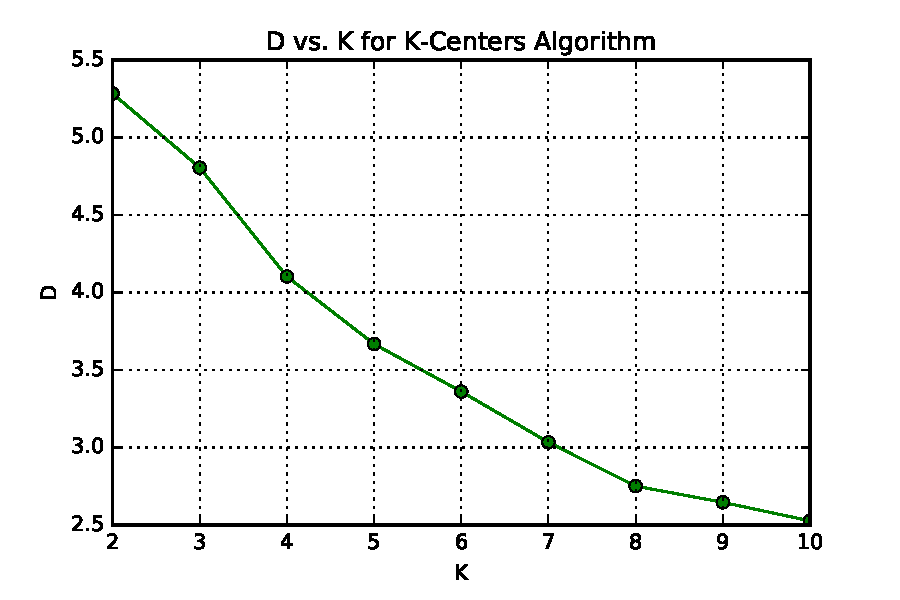
\includegraphics[width=\textwidth]{./figures/loss_clustering_kCenter.pdf}
            \caption{clustering.txt}\label{fig:4a}
        \end{subfigure}
        \hfill
        \begin{subfigure}[b]{0.49\textwidth}  
            \centering 
            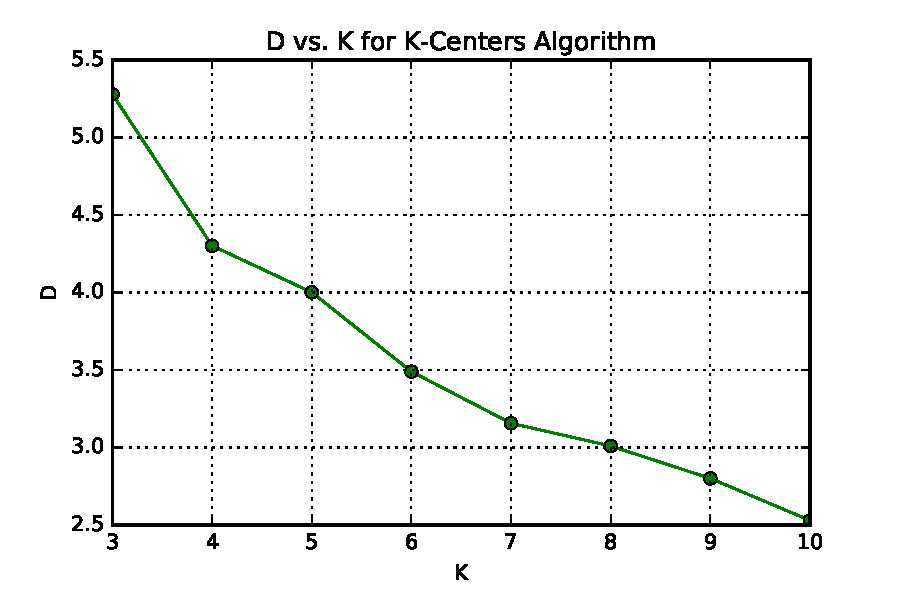
\includegraphics[width=\textwidth]{./figures/loss_bigClustering_kCenter.pdf}
            \caption{bigClusteringData.txt}\label{fig:4b}
        \end{subfigure}
\caption{Change of Distoration versus Cluster Number K for K-Center Algorithm}
\label{fig:k-centers-loss} 
\end{figure}

\item{2.} The scatter plot of the clustering result for clustering.txt is shown in Fig. \ref{fig:kcenter_clustering} and the scatter plot of the clustering result for bigClusteringData.txt is shown in Fig. \ref{fig:kcenter_bigClustering}. The cluster centroids are clearly marked and different clusters are denoted by different colors. 

%  -----------------------------------------------------------------------------
\begin{figure}[!h]
        \centering
        \begin{subfigure}[b]{0.475\textwidth}
            \centering
            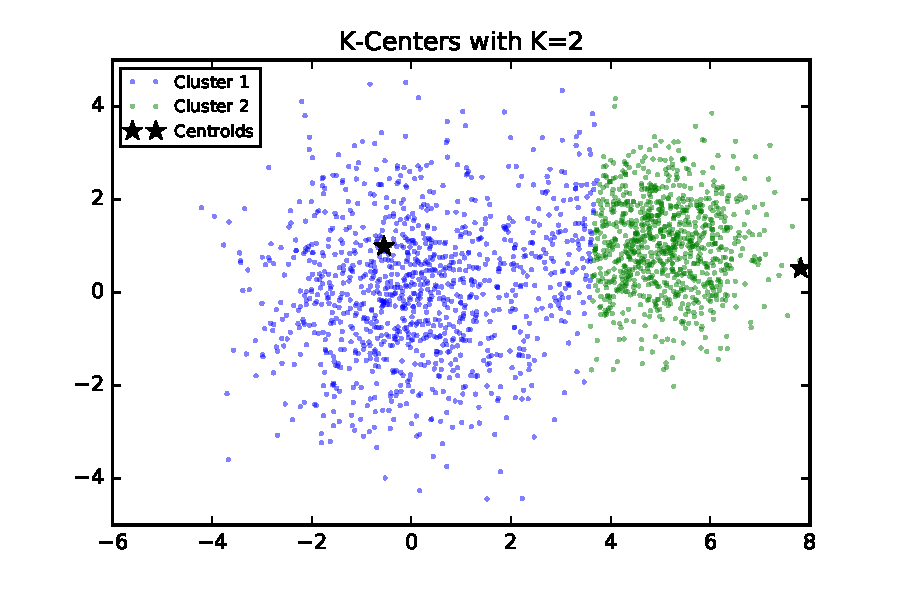
\includegraphics[width=\textwidth]{./figures/clustering_kCenter_2.pdf}
        \end{subfigure}
        \hfill
        \begin{subfigure}[b]{0.475\textwidth}  
            \centering 
            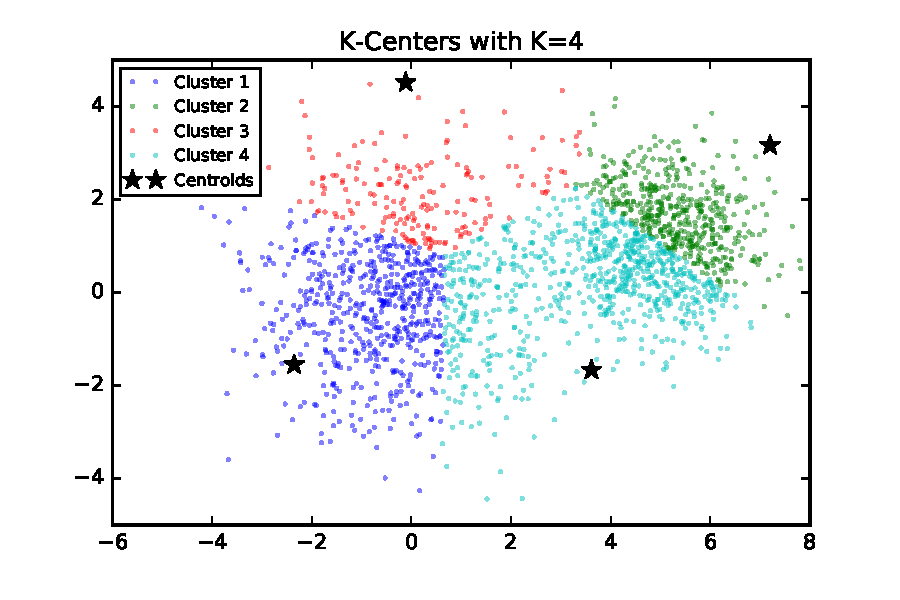
\includegraphics[width=\textwidth]{./figures/clustering_kCenter_4.pdf}
        \end{subfigure}      
        \caption{Clustering Result for clustering.txt with K-Center Algorithm}
        \label{fig:kcenter_clustering}
\end{figure}

%  -----------------------------------------------------------------------------
\begin{figure}[!h]
        \centering
        \begin{subfigure}[b]{0.475\textwidth}
            \centering
            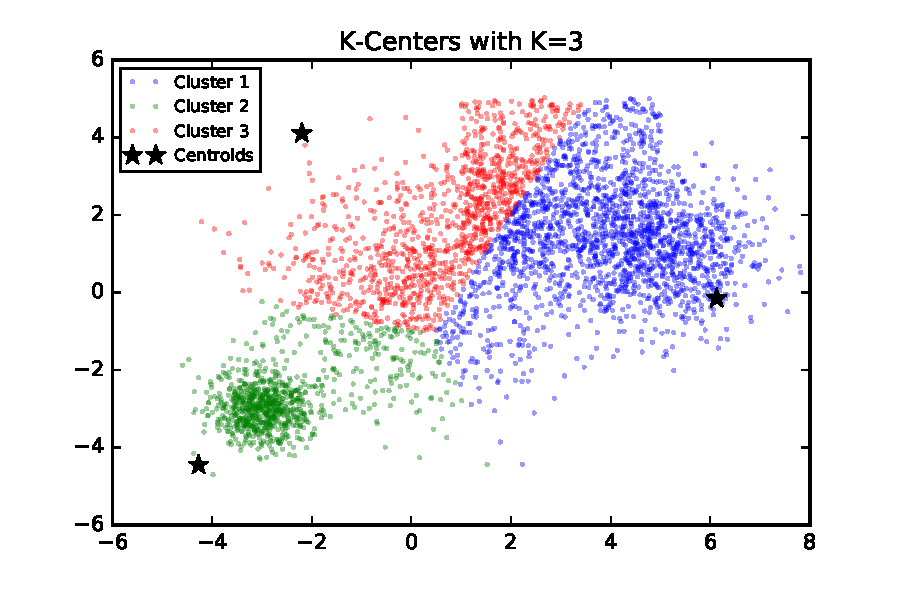
\includegraphics[width=\textwidth]{./figures/bigClustering_kCenter_3.pdf}
        \end{subfigure}
        \hfill      
        \begin{subfigure}[b]{0.475\textwidth}  
            \centering 
            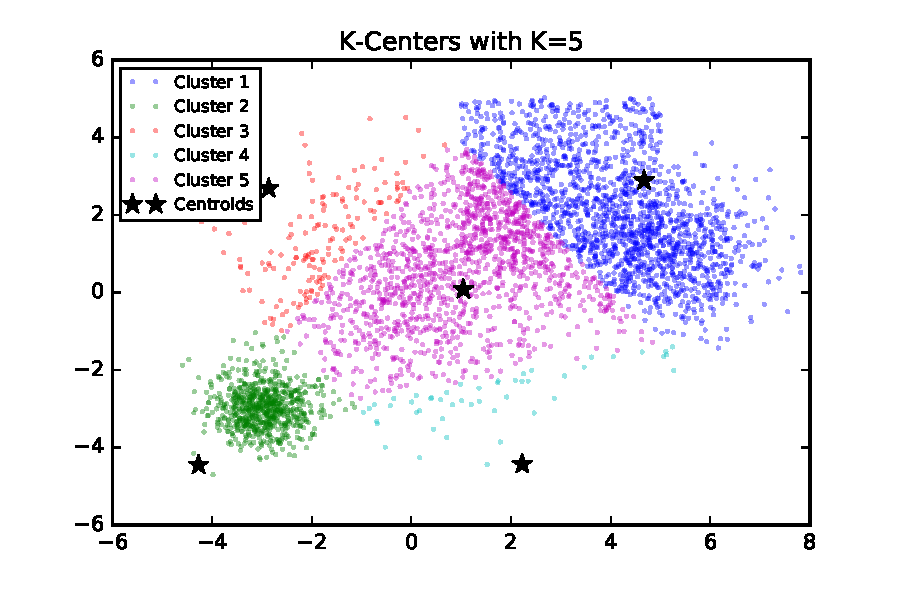
\includegraphics[width=\textwidth]{./figures/bigClustering_kCenter_5.pdf}
        \end{subfigure}  
        \begin{subfigure}[b]{0.475\textwidth}   
            \centering 
            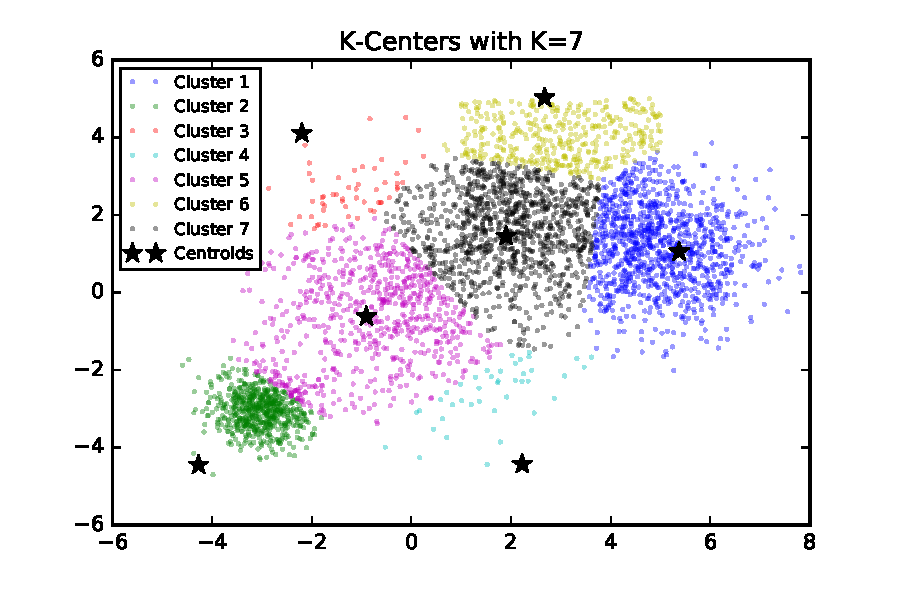
\includegraphics[width=\textwidth]{./figures/bigClustering_kCenter_7.pdf}
        \end{subfigure}
        \hfill
        \begin{subfigure}[b]{0.475\textwidth}   
            \centering 
            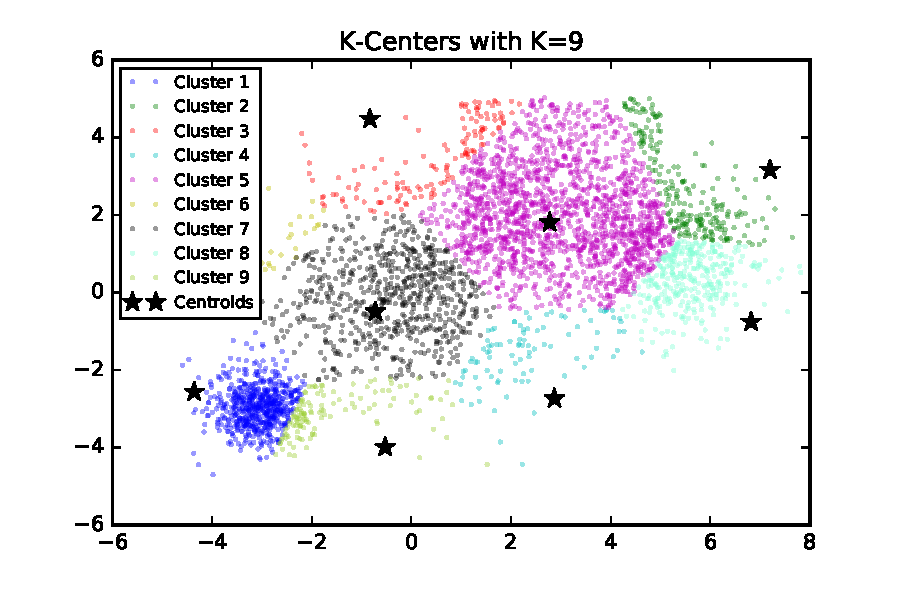
\includegraphics[width=\textwidth]{./figures/bigClustering_kCenter_9.pdf}
        \end{subfigure}
        
        \caption{Clustering Result for bigClusteringData.txt with K-Center Algorithm}
        \label{fig:kcenter_bigClustering}
\end{figure}

\newpage
\item{3.} The Python code used for K-Centers Algorithm is shown in Listing 2.

% -----------------------------------------------------------------------------
\begin{lstlisting}[language=Python, caption=K-Centers Algorithm Python Code]
import numpy as np
import time

def kCenters(X, K, random_state=None, verbose=True):
    """ function to implement the greedy k-centers algorithm """
    np.random.seed(random_state)
    t0 = time.time()

    N, d = X.shape
    # find the initial center
    index = np.random.choice(range(N), size=1)
    Q = np.zeros((K, d))
    Q[0, :] = X[index, :]
    idx = [index]

    i = 1
    while i < K:
        distance = np.zeros((N, i))
        for j in range(i):
            distance[:, j] = np.sum((X - Q[j, :])**2, axis=1)
        min_distance = np.min(distance, axis=1)
        new_index = np.argmax(min_distance)
        idx.append(new_index)
        Q[i, :] = X[new_index, :]
        i += 1

    loss = np.zeros((N, K))
    for i in range(K):
        loss[:, i] = np.sqrt(np.sum((X - Q[i, :])**2, axis=1))
    D = np.max(np.min(loss, axis=1))
    C = np.argmin(loss, axis=1)

    if verbose is True:
        t = np.round(time.time() - t0, 4)
        print('K-Centers is finished in ' + str(t) + 's')

    return Q, C, D, idx
\end{lstlisting}

% -----------------------------------------------------------------------------
\item{4.} Different Initialization Comparison.

In K-Centers algorithm, we run 50 times with different initialization, the best result of D is shown in Table \ref{table:best_kcenter}.

\begin{table}[H]
	\centering
	\caption{Best Result (D) for K-Centers Algorithm}
	\label{table:best_kcenter}	
	\begin{tabular}{ c | c | c | c | c | c | c | c | c | c}
		\hline \hline
		Data / K      & 2     &    3    & 4    & 5     & 6    & 7    & 8   & 9    & 10 \\[0.1cm]
		\hline
	clustering	        & 5.2838 &    4.8162 & 4.1387 & 3.7503 & 3.4691 & 3.1323 & 2.7510 & 2.7206 & 2.4634 \\[0.1cm]
bigClusteringData & N.A. &    5.5288 & 4.1446 & 3.8318 & 3.3765 & 3.2933 & 3.0093 & 2.7431 & 2.6249 \\[0.1cm]
		\hline	
	\end{tabular}
\end{table}

% -----------------------------------------------------------------------------
\item{5.} Cluster Index Comparison.

In K-Centers algorithm, the cluster index set C (first 20) for the best result is shown in Table \ref{table:index_kcenter_clustering} and Table \ref{table:index_kcenter_bigClustering}.

\begin{table}[H]
	\centering
	\caption{Index (first 20) for K-Centers Algorithm (clustering.txt)}
	\label{table:index_kcenter_clustering}	
	\begin{tabular}{ c | c }
		\hline \hline
		K        &    Index  \\[0.1cm]
		\hline
		2     &  0 0 0 0 0 0 0 0 0 0 0 0 0 0 0 0 0 0 0 0 \\[0.1cm]
		3     &  0 0 0 0 0 0 0 0 0 0 0 0 0 0 0 0 0 0 0 0 \\[0.1cm]
		4     &  2 2 1 2 1 3 3 2 3 2 3 2 3 3 2 3 3 2 2 3 \\[0.1cm]
		5     &  4 4 4 4 4 4 4 4 4 4 4 4 4 0 4 4 4 3 4 4 \\[0.1cm]
		6     &  5 5 5 5 5 5 5 3 5 5 5 5 5 5 3 5 5 3 5 5 \\[0.1cm]
		7     &  4 4 6 4 6 4 4 4 4 4 4 4 4 4 1 4 4 3 4 4 \\[0.1cm]
		8     &  6 6 6 6 0 0 0 6 0 6 0 6 0 5 6 0 0 2 6 0 \\[0.1cm]
		9     &  6 6 6 6 0 0 6 6 0 6 0 6 0 5 6 0 0 2 6 6 \\[0.1cm]
		10   &  6 6 6 6 6 6 6 6 6 6 6 6 5 5 0 6 6 8 6 6 \\[0.1cm]
		\hline	
	\end{tabular}
\end{table}

\begin{table}[H]
	\centering
	\caption{Index (first 20) for K-Centers Algorithm (bigClusteringData.txt)}
	\label{table:index_kcenter_bigClustering}	
	\begin{tabular}{ c | c }
		\hline \hline
		K    & Index \\[0.1cm]
		\hline
		3     &  1 0 0 0 0 0 0 0 0 0 0 0 1 1 0 0 2 0 2 0 \\[0.1cm]
		4     &  3 3 0 0 0 0 3 0 3 0 2 0 1 3 3 0 2 2 2 0 \\[0.1cm]
		5     &  3 3 4 0 0 4 3 4 3 4 2 0 1 3 3 0 2 2 2 0 \\[0.1cm]
		6     &  0 0 1 4 4 1 0 1 4 1 0 4 0 0 0 4 0 0 5 4 \\[0.1cm]
		7     &  5 5 2 5 0 6 5 2 5 2 5 6 4 1 5 6 4 5 0 6 \\[0.1cm]
		8     &  7 7 1 0 0 6 7 1 0 1 0 6 4 2 7 6 4 0 0 6 \\[0.1cm]
		9     &  7 4 8 4 4 8 4 1 4 1 4 6 0 7 4 4 5 4 5 4 \\[0.1cm]
		10   &  3 5 0 7 7 0 3 0 5 0 5 7 5 6 5 7 5 5 5 7 \\[0.1cm]
		\hline	
	\end{tabular}
\end{table}

\end{description}


% -----------------------------------------------------------------------------
\item[(\Romannum{3}).] Single-Swap Algorithm

\begin{description}
\item{1.} In this part, with the Single-Swap Algorithm for K-Centers clustering, we choose the best distortion D as the the objection function. Setting $\tau = 0.05$, the change of D versus cluster number K is shown in Fig. \ref{fig:single-swap-loss}, where the result for clustering.txt is shown in Fig. \ref{fig:7a} and the result for bigClusteringData.txt is show in Fig. \ref{fig:7b}.

%  -----------------------------------------------------------------------------
\begin{figure}[H]
\centering
\centering
        \begin{subfigure}[b]{0.49\textwidth}
            \centering
            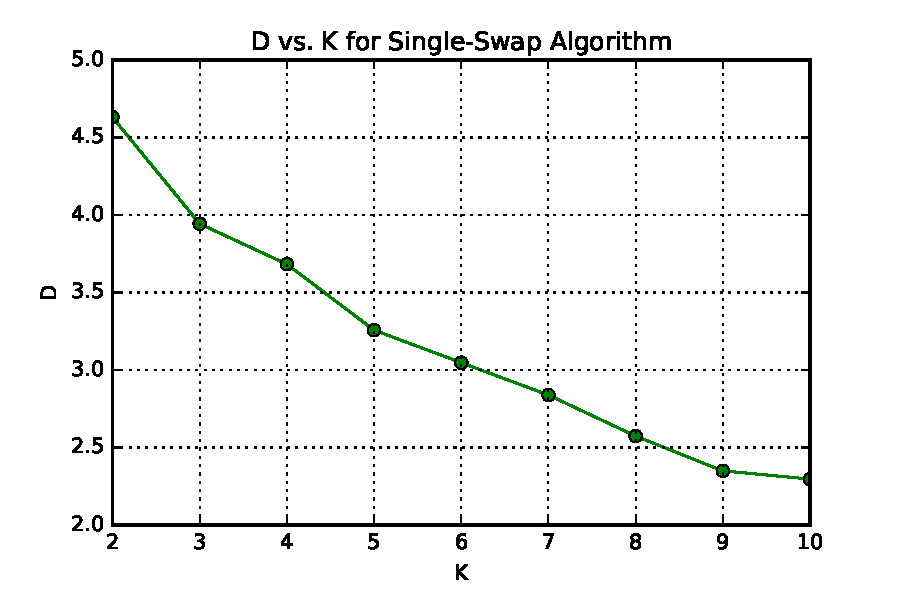
\includegraphics[width=\textwidth]{./figures/loss_clustering_singleSwap.pdf}
            \caption{clustering.txt}\label{fig:7a}
        \end{subfigure}
        \hfill
        \begin{subfigure}[b]{0.49\textwidth}  
            \centering 
            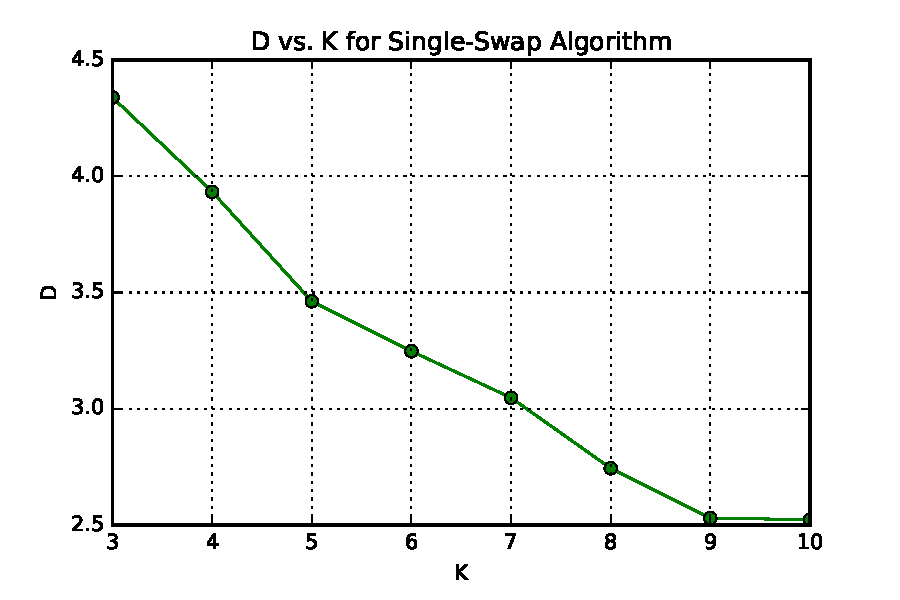
\includegraphics[width=\textwidth]{./figures/loss_bigClustering_singleSwap.pdf}
            \caption{bigClusteringData.txt}\label{fig:7b}
        \end{subfigure}
\caption{Change of Distoration versus Cluster Number K for Single-Swap Algorithm}
\label{fig:single-swap-loss} 
\end{figure}

\item{2.} The scatter plot of the clustering result for clustering.txt is shown in Fig. \ref{fig:single-swap-clusterimg} and the scatter plot of the clustering result for bigClusteringData.txt is shown in Fig. \ref{fig:single-swap-bigClustering}. The cluster centroids are clearly marked and different clusters are denoted by different colors. 

%  -----------------------------------------------------------------------------
\begin{figure}[!h]
        \centering
        \begin{subfigure}[b]{0.475\textwidth}
            \centering
            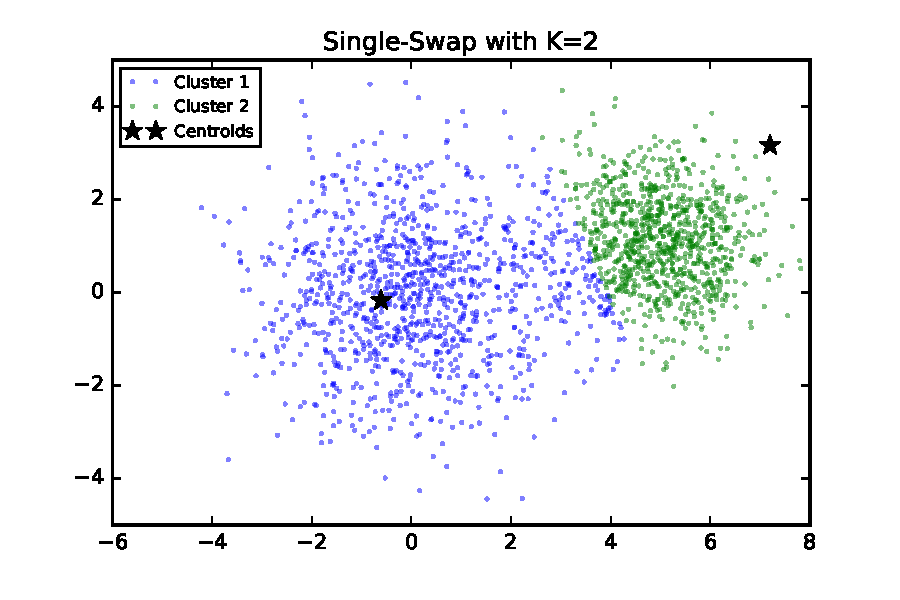
\includegraphics[width=\textwidth]{./figures/clustering_singleSwap_2.pdf}
        \end{subfigure}
        \hfill
        \begin{subfigure}[b]{0.475\textwidth}  
            \centering 
            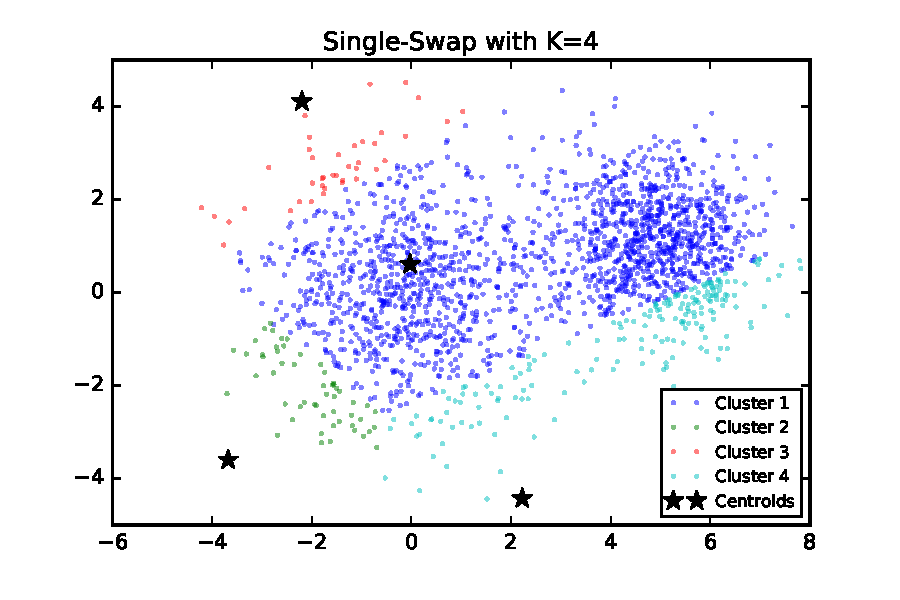
\includegraphics[width=\textwidth]{./figures/clustering_singleSwap_4.pdf}
        \end{subfigure}        
        \caption{Clustering Result for clustering.txt with Single-Swap Algorithm}
        \label{fig:single-swap-clusterimg}
\end{figure}

%  -----------------------------------------------------------------------------
\begin{figure}[!h]
        \centering
        \begin{subfigure}[b]{0.475\textwidth}
            \centering
            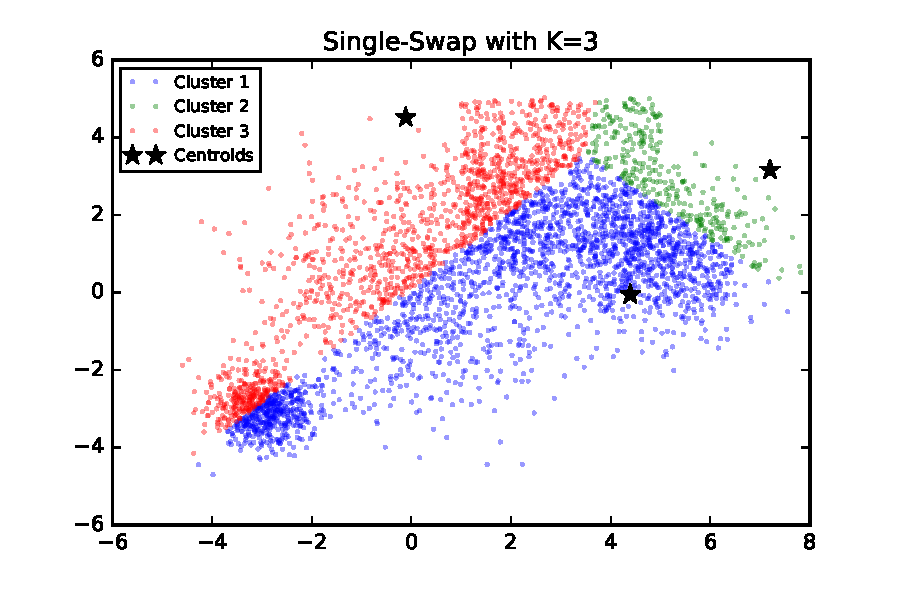
\includegraphics[width=\textwidth]{./figures/bigClustering_singleSwap_3.pdf}
        \end{subfigure}
        \hfill    
        \begin{subfigure}[b]{0.475\textwidth}  
            \centering 
            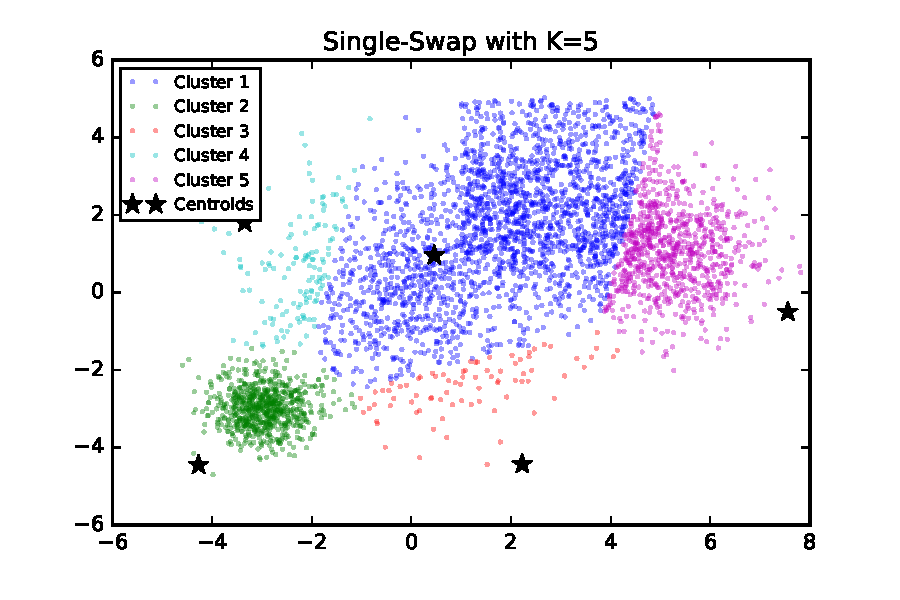
\includegraphics[width=\textwidth]{./figures/bigClustering_singleSwap_5.pdf}
        \end{subfigure}
        \begin{subfigure}[b]{0.475\textwidth}   
            \centering 
            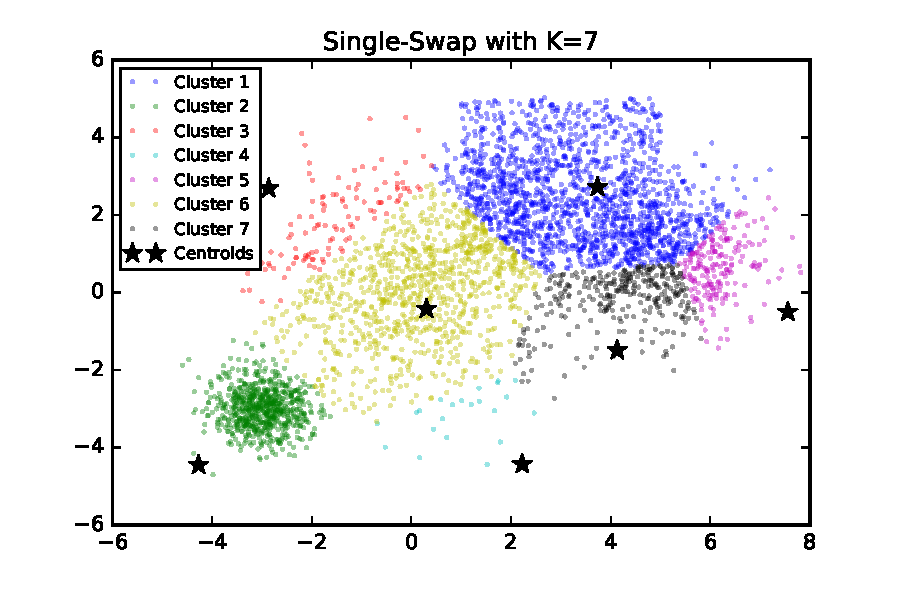
\includegraphics[width=\textwidth]{./figures/bigClustering_singleSwap_7.pdf}
        \end{subfigure}
        \hfill
        \begin{subfigure}[b]{0.475\textwidth}   
            \centering 
            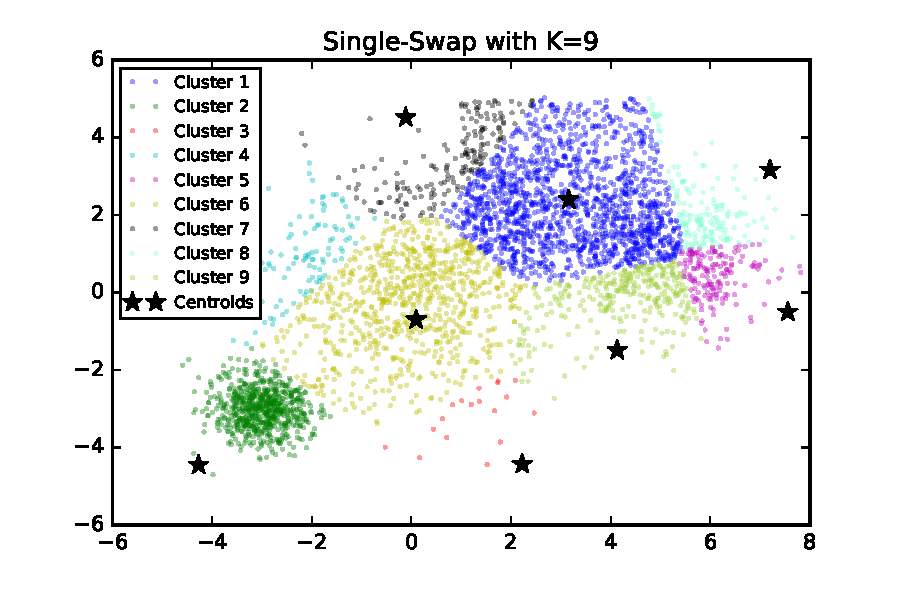
\includegraphics[width=\textwidth]{./figures/bigClustering_singleSwap_9.pdf}
        \end{subfigure}
        
        \caption{Clustering Result for bigClusteringData.txt with Single-Swap Algorithm}
        \label{fig:single-swap-bigClustering}
\end{figure}


\newpage
\item{3.} The Python code used for Single-Swap Algorithm is shown in Listing 3.

% -----------------------------------------------------------------------------
\begin{lstlisting}[language=Python, caption=Single-Swap Algorithm Python Code]
import numpy as np
import time
from k_centers import kCenters

def singleSwap(X, K, tau=0.05, random_state=None, verbose=True):
    """ function to implement the single-swap for k-centers algorithm """
    t0 = time.time()

    # calculate the initial centers
    Q, _, pre_cost, _ = kCenters(X, K, random_state=random_state,
                                 verbose=False)
    N, d = X.shape

    # compute the distance based on current centers
    distance = np.zeros((N, K))
    for idx in range(K):
        distance[:, idx] = np.sqrt(np.sum((X - Q[idx, :])**2, axis=1))
    cost = np.max(np.min(distance, axis=1))  # calculate cost

    i = 0
    while i < K:
        if i == 0:
            min_dist = np.min(distance[:, 0:], axis=1)
        elif i == (K - 1):
            min_dist = np.min(distance[:, :-1], axis=1)
        else:
            min_dist = np.minimum(np.min(distance[:, :i], axis=1),
                                  np.min(distance[:, (i + 1):], axis=1))
        swap = False  # keep recording whether or not swaped
        for j in range(N):
            tmp_dist = np.sqrt(np.sum((X - X[j, :])**2, axis=1))
            new_cost = np.max(np.minimum(min_dist, tmp_dist))
            if new_cost / cost < (1 - tau):
                Q[i, :] = X[j, :]
                distance[:, i] = tmp_dist
                swap = True
                cost = new_cost
        i += 1

        if swap is False:
            if i == K - 1:
                break
            else:
                i += 1
        elif (swap is True) and (i == K):
            i = 0

    C = np.argmin(distance, axis=1)

    if verbose is True:
        t = np.round(time.time() - t0, 4)
        print('Single-Swap is finished in ' + str(t) + 's')

    return Q, C, cost
\end{lstlisting}

% -----------------------------------------------------------------------------
\item{4.} Different Initialization Comparison.

In Single-Swap algorithm, we run 50 times with different initialization, the best result of D is shown in Table \ref{table:best_single}.

\begin{table}[H]
	\centering
	\caption{Best Result (D) for Single-Swap Algorithm}
	\label{table:best_single}	
	\begin{tabular}{ c | c | c | c | c | c | c | c | c | c}
		\hline \hline
		Data / K      & 2     &    3    & 4    & 5     & 6    & 7    & 8   & 9    & 10 \\[0.1cm]
		\hline
	clustering	        & 4.6305 &    3.9619 & 3.7152 & 3.3236 & 3.0420 & 2.8479 & 2.5808 & 2.3493 & 2.3493 \\[0.1cm]
bigClusteringData & N.A. &    4.3388 & 3.8504 & 3.4619 & 3.2156 & 2.9379 & 2.8479 & 2.6053 & 2.4973 \\[0.1cm]
		\hline	
	\end{tabular}
\end{table}

% -----------------------------------------------------------------------------
\item{5.} Cluster Index Comparison.

In Single-Swap algorithm, the cluster index set C (first 20) for the best result is shown in Table \ref{table:index_single_clustering} and Table \ref{table:index_single_bigClustering}.

\begin{table}[H]
	\centering
	\caption{Index (first 20) for Single-Swap Algorithm (clustering.txt)}
	\label{table:index_single_clustering}	
	\begin{tabular}{ c | c }
		\hline \hline
		K        &    Index  \\[0.1cm]
		\hline
		2   & 0 0 0 0 0 0 0 0 0 0 0 0 0 0 0 0 0 0 0 0 \\[0.1cm]
	    3   & 0 0 0 0 2 0 0 0 0 0 0 0 0 0 0 0 0 0 0 0 \\[0.1cm]
        4   & 0 0 0 2 0 0 0 2 0 0 0 0 0 0 2 0 0 2 0 0 \\[0.1cm]
        5   & 4 4 4 4 4 4 4 4 4 4 4 4 4 4 4 4 4 3 4 4 \\[0.1cm]
        6   & 0 0 3 0 5 0 0 0 0 0 0 0 4 0 2 0 0 2 0 0 \\[0.1cm]
        7   & 6 6 6 6 6 6 6 6 0 6 0 6 4 0 3 6 6 6 6 0 \\[0.1cm]
        8   & 7 7 0 7 0 7 7 7 7 7 7 7 5 5 4 7 7 4 7 7 \\[0.1cm]
        9   & 4 4 4 4 0 4 4 4 4 4 4 4 3 8 2 4 4 2 4 4 \\[0.1cm]
        10 & 4 4 4 4 8 4 4 4 9 4 4 4 3 9 2 4 4 2 4 4 \\[0.1cm]
		\hline	
	\end{tabular}
\end{table}

\begin{table}[H]
	\centering
	\caption{Index (first 20) for Single-Swpa Algorithm (bigClusteringData.txt)}
	\label{table:index_single_bigClustering}	
	\begin{tabular}{ c | c }
		\hline \hline
		K    & Index \\[0.1cm]
		\hline
		3     &  0 0 1 0 0 1 0 1 0 1 0 2 0 0 0 0 0 0 0 0 \\[0.1cm]
		4     &  3 3 0 0 0 0 3 0 3 0 2 0 1 3 3 0 2 2 2 0 \\[0.1cm]
		5     &  0 0 1 0 0 1 0 1 0 1 0 0 4 3 0 0 4 0 4 0 \\[0.1cm]
		6     &  5 5 1 5 5 1 5 1 5 1 5 0 4 5 5 5 4 5 4 5 \\[0.1cm]
		7     &  5 4 0 4 4 0 4 0 4 0 4 2 1 5 4 4 1 4 6 4 \\[0.1cm]
		8     &  7 0 3 0 0 3 0 3 0 3 0 6 1 5 0 0 7 0 4 0 \\[0.1cm]
		9     &  4 4 8 6 6 8 4 8 4 8 4 6 0 7 4 6 0 4 4 6 \\[0.1cm]
		10   &  4 4 0 7 7 0 3 0 4 0 4 7 4 6 4 7 4 4 2 7 \\[0.1cm]
		\hline	
	\end{tabular}
\end{table}

\end{description}


% -----------------------------------------------------------------------------
\item[(\Romannum{4}).] Spectral Clustering Algorithm

\begin{description}
\item{1.} In this part, with the Spectral Clustering Algorithm, we choose the best distortion D as the the objection function and using Euclidean distance between points to construct the W matrix. Then, using the first k-eigenvectors as the input to Greedy K-Centers algortihm, the change of D versus cluster number K is shown in Fig. \ref{fig:spectral-loss}, where the result for clustering.txt is shown in Fig. \ref{fig:10a} and the result for bigClusteringData.txt is show in Fig. \ref{fig:10b}.

%  -----------------------------------------------------------------------------
\begin{figure}[H]
\centering
\centering
        \begin{subfigure}[b]{0.49\textwidth}
            \centering
            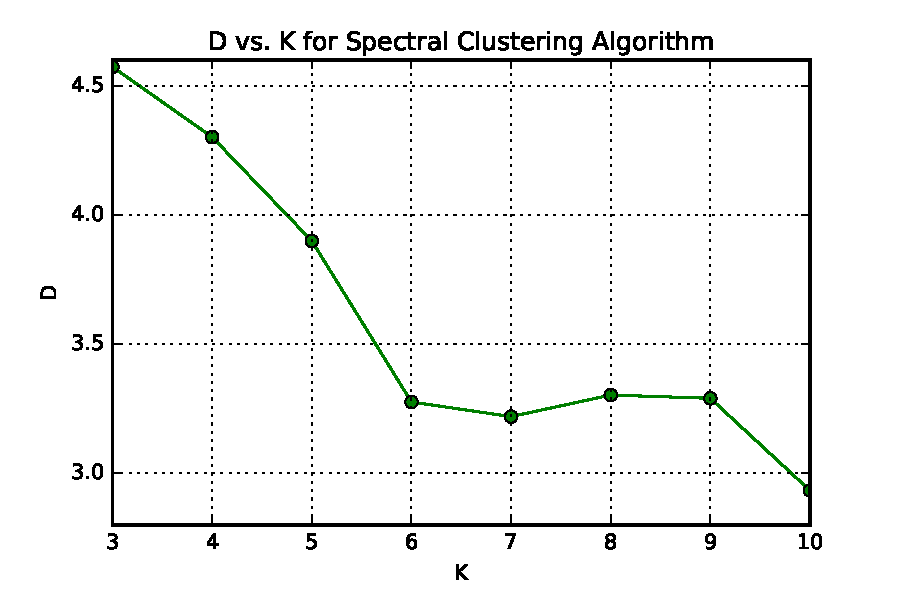
\includegraphics[width=\textwidth]{./figures/loss_clustering_spectral.pdf}
            \caption{clustering.txt}\label{fig:10a}
        \end{subfigure}
        \hfill
        \begin{subfigure}[b]{0.49\textwidth}  
            \centering 
            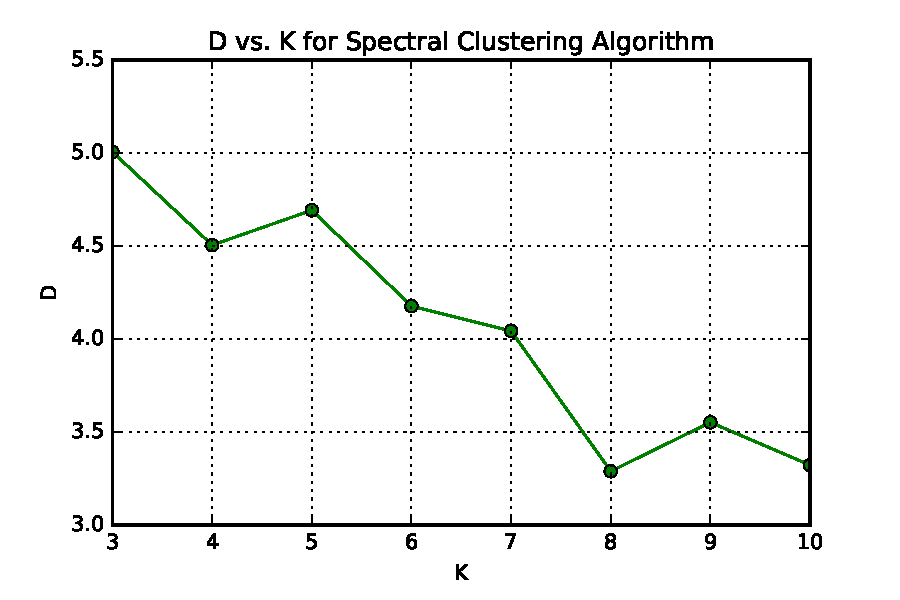
\includegraphics[width=\textwidth]{./figures/loss_bigClustering_spectral.pdf}
            \caption{bigClusteringData.txt}\label{fig:10b}
        \end{subfigure}
\caption{Change of Distoration versus Cluster Number K for Spectral Clustering}
\label{fig:spectral-loss} 
\end{figure}

Note: in above part, in order to calculate the cost $D = \underset{x_i \in X}{\max}( \underset{c_j \in Q}{\min}{||x_i - c_j||_2})$, we actually implement the Greedy K-Centers algorithm, rather than K-Means algorithm. However, the result of K-Centers algorithm is very bad. In the following part, we implement K-Means algorithm for actual clustering. \\


\item{2.} The scatter plot of the clustering result for clustering.txt is shown in Fig. \ref{fig:spectral_clustering} and the scatter plot of the clustering result for bigClusteringData.txt is shown in Fig. \ref{fig:spectral_bigClustering}. The cluster centroids are clearly marked and different clusters are denoted by different colors. 

%  -----------------------------------------------------------------------------
\begin{figure}[!h]
        \centering
        \begin{subfigure}[b]{0.475\textwidth}
            \centering
            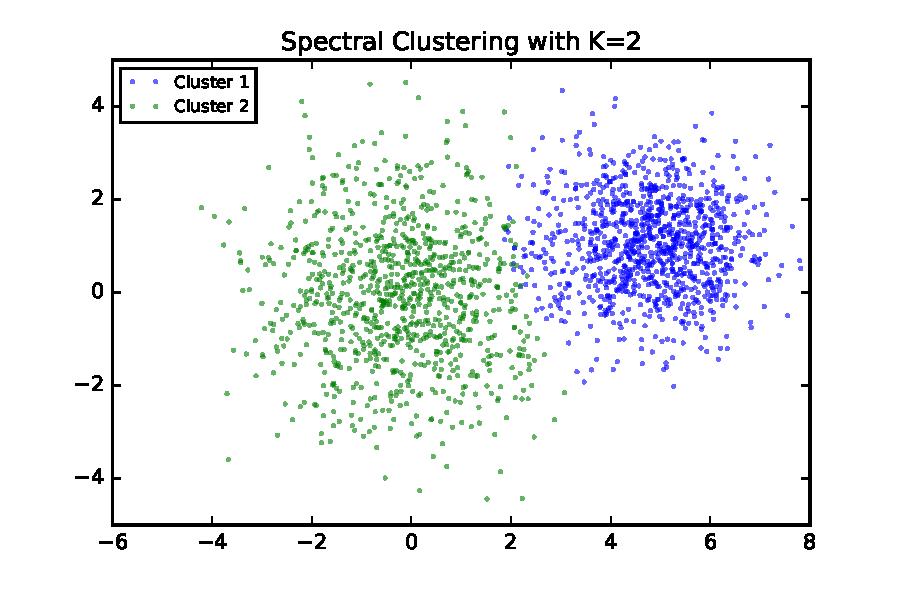
\includegraphics[width=\textwidth]{./figures/clustering_spectral_2.pdf}
        \end{subfigure}
        \hfill
        \begin{subfigure}[b]{0.475\textwidth}  
            \centering 
            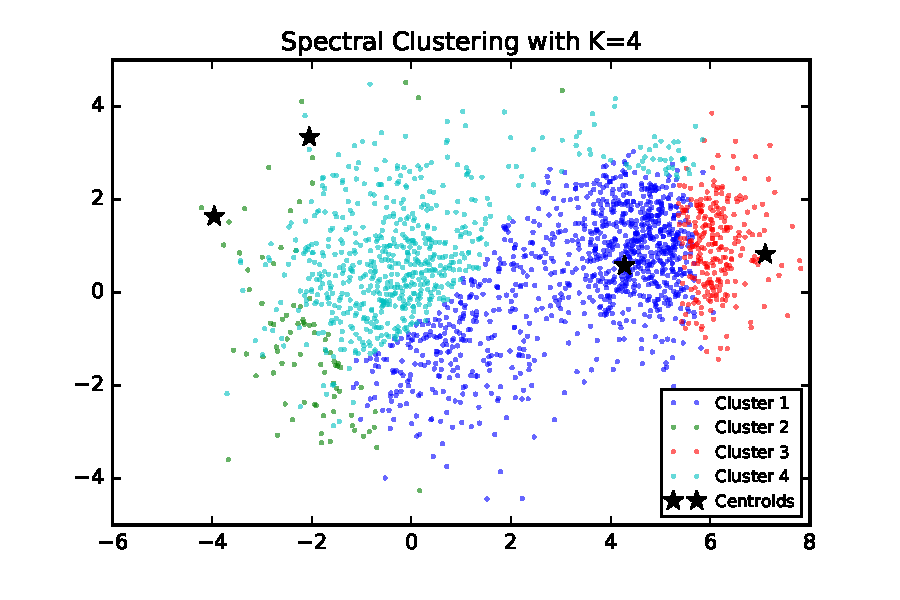
\includegraphics[width=\textwidth]{./figures/clustering_spectral_4.pdf}
        \end{subfigure}        
        \caption{Clustering Result for clustering.txt with Spectral Clustering}
        \label{fig:spectral_clustering}
\end{figure}

%  -----------------------------------------------------------------------------
\begin{figure}[!h]
        \centering
        \begin{subfigure}[b]{0.475\textwidth}
            \centering
            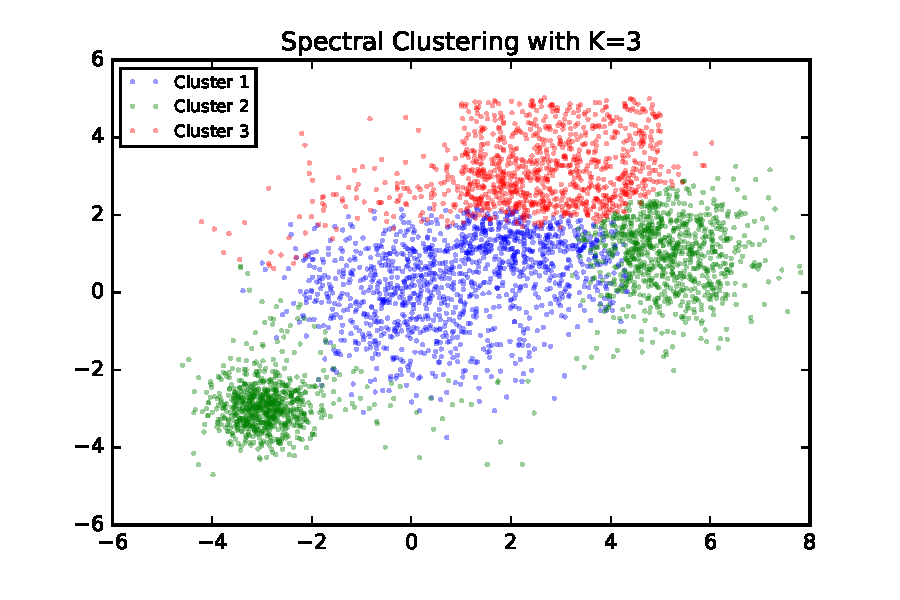
\includegraphics[width=\textwidth]{./figures/bigClustering_spectral_3.pdf}
        \end{subfigure}
        \hfill  
        \begin{subfigure}[b]{0.475\textwidth}  
            \centering 
            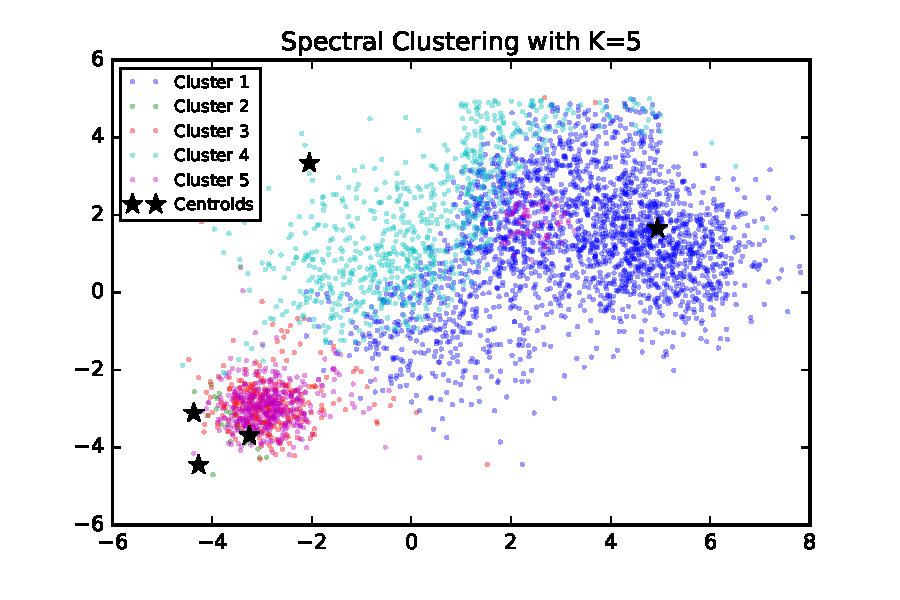
\includegraphics[width=\textwidth]{./figures/bigClustering_spectral_5.pdf}
        \end{subfigure}  
        \begin{subfigure}[b]{0.475\textwidth}   
            \centering 
            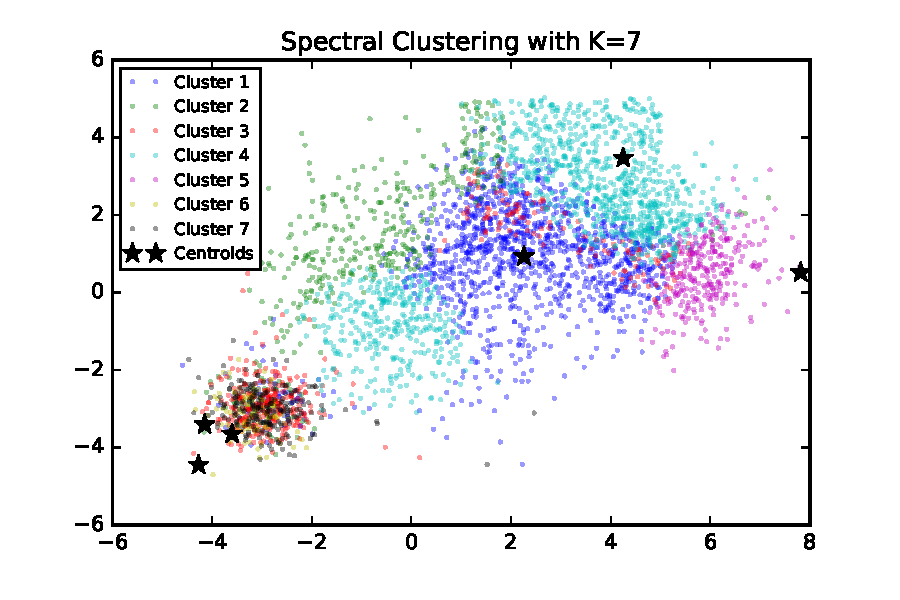
\includegraphics[width=\textwidth]{./figures/bigClustering_spectral_7.pdf}
        \end{subfigure}
        \hfill
        \begin{subfigure}[b]{0.475\textwidth}   
            \centering 
            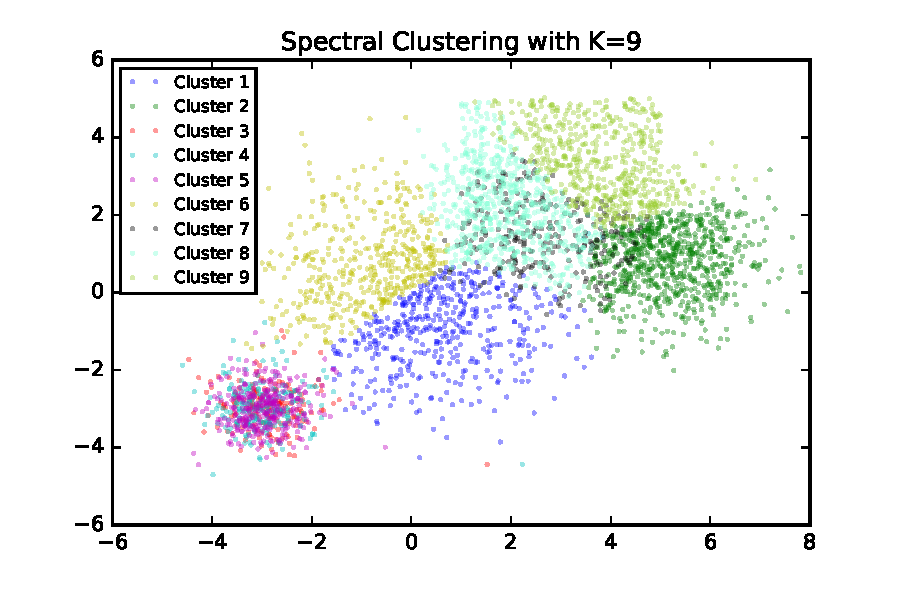
\includegraphics[width=\textwidth]{./figures/bigClustering_spectral_9.pdf}
        \end{subfigure}
        
        \caption{Clustering Result for bigClusteringData.txt with Spectral Clustering}
        \label{fig:spectral_bigClustering}
\end{figure}

\newpage
\item{3.} The Python code used for Spectral Clustering Algorithm is shown in Listing 4.

% -----------------------------------------------------------------------------
\begin{lstlisting}[language=Python, caption=Spectral Clustering Algorithm Python Code]
import numpy as np
import time
# from k_centers import kCenters
from k_means import kMeans


def spectralClustering(X, K, random_state=None, verbose=True):
    """ function to implement the spectral clustering algorithm """
    t0 = time.time()

    N, d = X.shape
    W = np.zeros((N, N))  # adjacency matrix W
    for i in range(N):
        distance = np.sqrt(np.sum((X - X[i, :])**2, axis=1))
        W[:, i] = distance

    diag = np.sum(W, axis=1)
    D = np.diag(diag)  # diagnoal matrix D
    L = D - W  # Laplacian matrix L
    L = np.identity(N) - np.dot(np.linalg.inv(D), W)
    eigvals, U = np.linalg.eigh(L)

    U = U[:, -K:]  # first K eigenvectors

    # # call k-centers for clustering
    # _, C, _, idx = kCenters(U, K, random_state=random_state, verbose=False)
    #
    # Q = X[idx, :]
    # loss = np.zeros((N, K))
    # for i in range(K):
    #     loss[:, i] = np.sqrt(np.sum((X - Q[i, :])**2, axis=1))
    # D = np.max(np.min(loss, axis=1))
    #
    # if verbose is True:
    #     t = np.round(time.time() - t0, 4)
    #     print('Spectral Clustering finished in ' + str(t) + 's')
    #
    # return W, U, Q, C, D

    # call k-means for clustering
    Q, C, D = kMeans(U, K, tol=0.00001, random_state=random_state,
                     verbose=False)

    if verbose is True:
        t = np.round(time.time() - t0, 4)
        print('Spectral Clustering finished in ' + str(t) + 's')

    return W, U, Q, C, D
\end{lstlisting}


% -----------------------------------------------------------------------------
\item{4.} Different Initialization Comparison.

In Spectral Clustering algorithm, we run 50 times with different initialization, the best result of D is shown in Table \ref{table:best_spectral}.

\begin{table}[H]
	\centering
	\caption{Best Result (D) for Spectral Clustering Algorithm}
	\label{table:best_spectral}	
	\begin{tabular}{ c | c | c | c | c | c | c | c | c | c}
		\hline \hline
		Data / K      & 2     &    3    & 4    & 5     & 6    & 7    & 8   & 9    & 10 \\[0.1cm]
		\hline
	clustering	        & 5.4780 &    4.8812 & 4.6889 & 3.7015 & 3.3656 & 3.3084 & 3.4417 & 3.1799 & 3.3345 \\[0.1cm]
bigClusteringData & N.A. &    5.0057 & 4.7021 & 4.2090 & 4.6857 & 3.6327 & 3.3554 & 3.5176 & 3.7858 \\[0.1cm]
		\hline	
	\end{tabular}
\end{table}

% -----------------------------------------------------------------------------
\item{5.} Cluster Index Comparison.

In Spectral Clustering algorithm, the cluster index set C (first 20) for the best result is shown in Table \ref{table:index_spectral_clustering} and Table \ref{table:index_spectral_bigClustering}.

\begin{table}[H]
	\centering
	\caption{Index (first 20) for Spectral Clustering Algorithm (clustering.txt)}
	\label{table:index_spectral_clustering}	
	\begin{tabular}{ c | c }
		\hline \hline
		K        &    Index  \\[0.1cm]
		\hline
		2     &  1.  1.  0.  1.  0.  0.  0.  1.  0.  1.  0.  1.  0.  0.  1.  0.  0.  1.  1.  0. \\[0.1cm]
		3     &  1.  1.  1.  1.  1.  1.  1.  1.  0.  1.  1.  0.  1.  0.  1.  1.  1.  1.  1.  0. \\[0.1cm]
		4     &  3.  3.  3.  3.  3.  2.  2.  3.  2.  2.  2.  2.  0.  0.  3.  2.  2.  3.  2.  2. \\[0.1cm]
		5     &  0.  2.  2.  0.  1.  1.  1.  0.  1.  0.  1.  0.  1.  1.  2.  1.  1.  2.  1.  1. \\[0.1cm]
		6     &  0.  0.  0.  0.  4.  0.  0.  2.  4.  0.  4.  1.  4.  4.  2.  4.  4.  2.  0.  1. \\[0.1cm]
		7     &  1.  6.  6.  6.  4.  6.  6.  1.  4.  6.  4.  1.  4.  4.  1.  4.  4.  1.  6.  6. \\[0.1cm]
		8     &  5.  2.  2.  5.  2.  5.  5.  4.  1.  5.  1.  5.  1.  1.  4.  1.  1.  4.  5.  1. \\[0.1cm]
		9     &  4.  5.  5.  5.  2.  2.  2.  4.  3.  4.  2.  4.  0.  3.  4.  2.  2.  4.  5.  2. \\[0.1cm]
		10   &  3.  5.  5.  5.  4.  5.  5.  0.  4.  5.  4.  3.  4.  4.  0.  4.  4.  3.  5.  4. \\[0.1cm]
		\hline	
	\end{tabular}
\end{table}

\begin{table}[H]
	\centering
	\caption{Index (first 20) for Spectral Clustering Algorithm (bigClusteringData.txt)}
	\label{table:index_spectral_bigClustering}	
	\begin{tabular}{ c | c }
		\hline \hline
		K    & Index \\[0.1cm]
		\hline
		3     &  0.  2.  0.  2.  2.  0.  2.  0.  2.  0.  2.  2.  0.  0.  2.  2.  1.  2.  1.  2. \\[0.1cm]
		4     &  3.  1.  2.  1.  1.  2.  1.  2.  1.  2.  1.  2.  3.  3.  1.  1.  2.  1.  2.  1. \\[0.1cm]
		5     &  0.  1.  3.  4.  4.  3.  4.  3.  4.  3.  1.  4.  0.  0.  4.  4.  1.  1.  1.  4. \\[0.1cm]
		6     &  4.  4.  1.  5.  5.  1.  4.  1.  4.  1.  4.  5.  2.  5.  4.  5.  2.  4.  2.  5. \\[0.1cm]
		7     &  3.  1.  5.  4.  4.  5.  1.  5.  1.  5.  1.  4.  3.  3.  1.  4.  2.  1.  2.  4. \\[0.1cm]
		8     &  2.  4.  7.  4.  4.  7.  1.  7.  4.  7.  4.  0.  5.  2.  4.  1.  5.  4.  4.  1. \\[0.1cm]
		9     &  5.  4.  1.  4.  8.  1.  0.  1.  4.  1.  4.  8.  3.  5.  4.  0.  1.  4.  1.  0. \\[0.1cm]
		10   &  2.  1.  4.  1.  3.  4.  7.  4.  1.  4.  1.  3.  6.  2.  1.  7.  6.  1.  8.  7. \\[0.1cm]
		\hline	
	\end{tabular}
\end{table}

\end{description}


% -----------------------------------------------------------------------------
\item[(\Romannum{5}).] Expectation Maximization (EM) Algorithm

\begin{description}
\item{1.} In this part, assuming we are dealing with the Gaussian Mixture Model (GMM), then with the EM algorithm, we choose the best distortion D as the the objection function. The change of D versus cluster number K is shown in Fig. \ref{fig:EM-loss}, where the result for clustering.txt is shown in Fig. \ref{fig:13a} and the result for bigClusteringData.txt is show in Fig. \ref{fig:13b}.

%  -----------------------------------------------------------------------------
\begin{figure}[H]
\centering
\centering
        \begin{subfigure}[b]{0.49\textwidth}
            \centering
            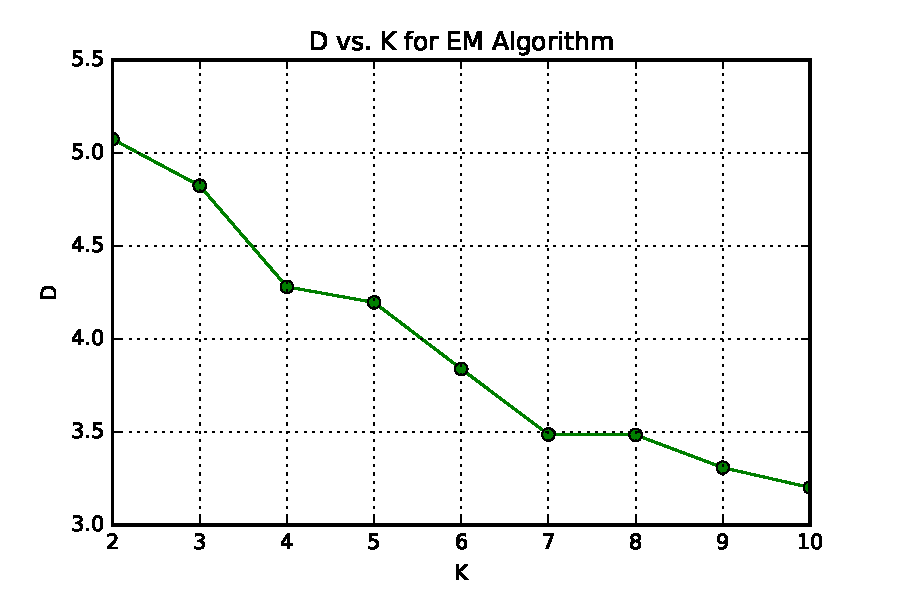
\includegraphics[width=\textwidth]{./figures/loss_clustering_EM.pdf}
            \caption{clustering.txt}\label{fig:13a}
        \end{subfigure}
        \hfill
        \begin{subfigure}[b]{0.49\textwidth}  
            \centering 
            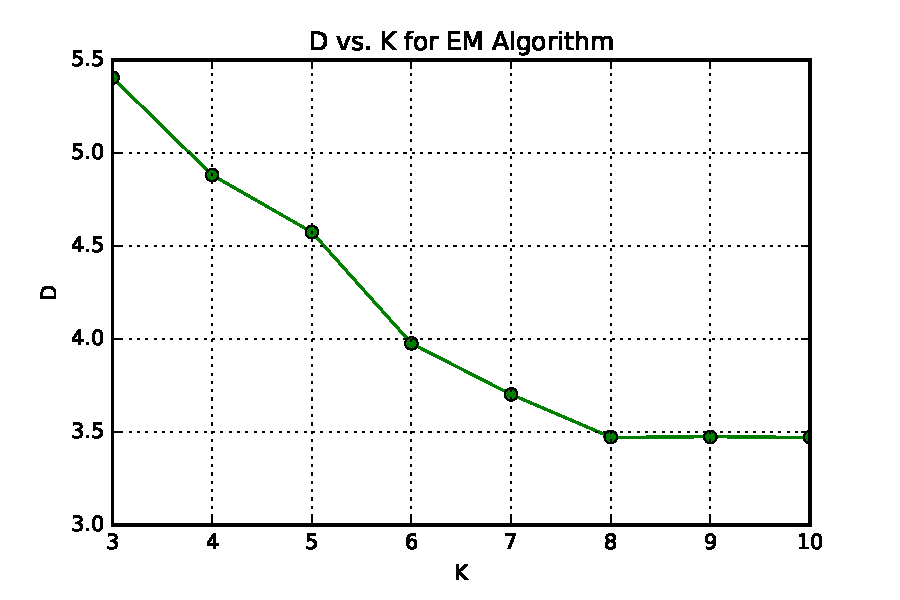
\includegraphics[width=\textwidth]{./figures/loss_bigClustering_EM.pdf}
            \caption{bigClusteringData.txt}\label{fig:13b}
        \end{subfigure}
\caption{Change of Distoration versus Cluster Number K for EM Algorithm}
\label{fig:EM-loss} 
\end{figure}

\item{2.} The scatter plot of the clustering result for clustering.txt is shown in Fig. \ref{fig:EM_clustering} and the scatter plot of the clustering result for bigClusteringData.txt is shown in Fig. \ref{fig:EM_bigClustering}. The cluster centroids are clearly marked and different clusters are denoted by different colors. 

%  -----------------------------------------------------------------------------
\begin{figure}[!h]
        \centering
        \begin{subfigure}[b]{0.475\textwidth}
            \centering
            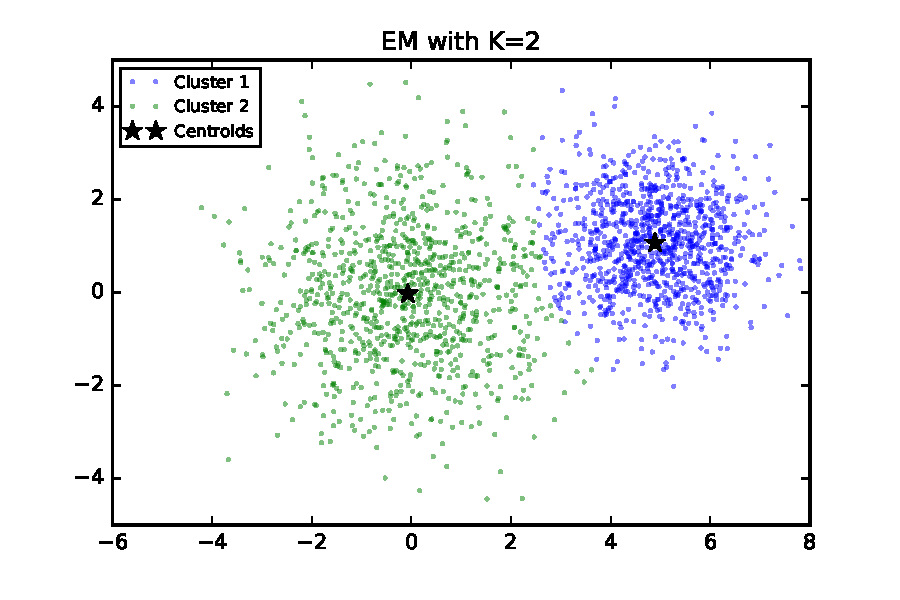
\includegraphics[width=\textwidth]{./figures/clustering_EM_2.pdf}
        \end{subfigure}
        \hfill
        \begin{subfigure}[b]{0.475\textwidth}  
            \centering 
            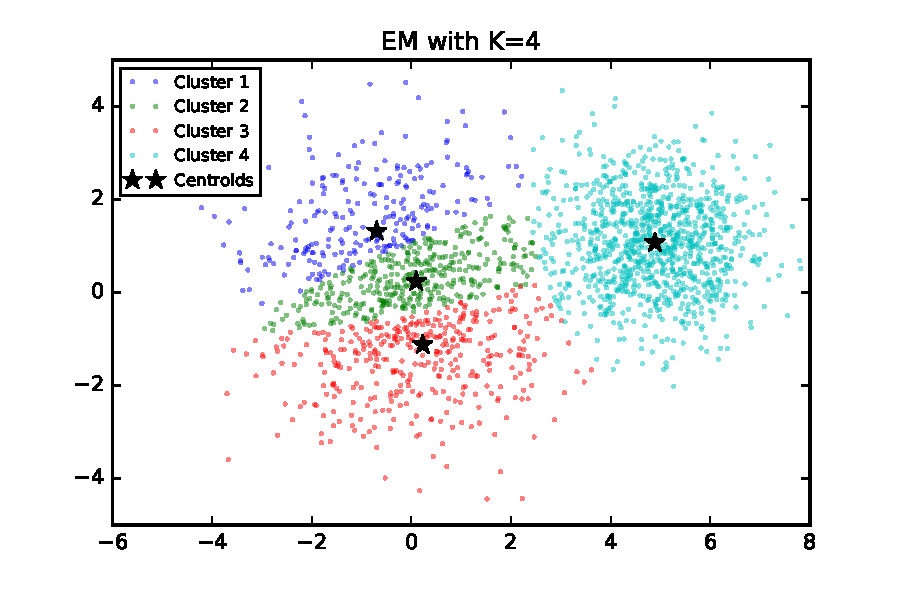
\includegraphics[width=\textwidth]{./figures/clustering_EM_4.pdf}
        \end{subfigure}       
        \caption{Clustering Result for clustering.txt with EM Algorithm}
        \label{fig:EM_clustering}
\end{figure}

%  -----------------------------------------------------------------------------
\begin{figure}[!h]
        \centering
        \begin{subfigure}[b]{0.475\textwidth}
            \centering
            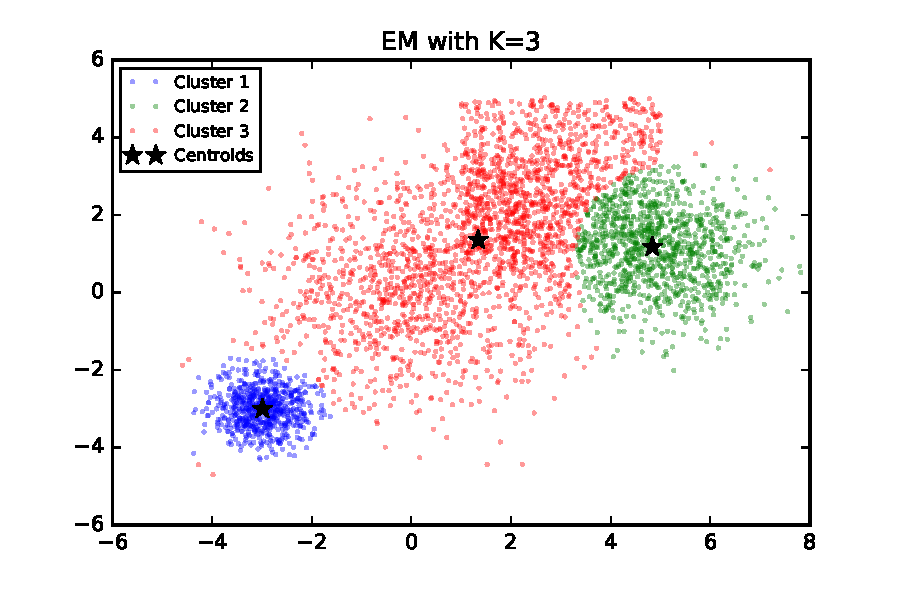
\includegraphics[width=\textwidth]{./figures/bigClustering_EM_3.pdf}
        \end{subfigure}
        \hfill      
        \begin{subfigure}[b]{0.475\textwidth}  
            \centering 
            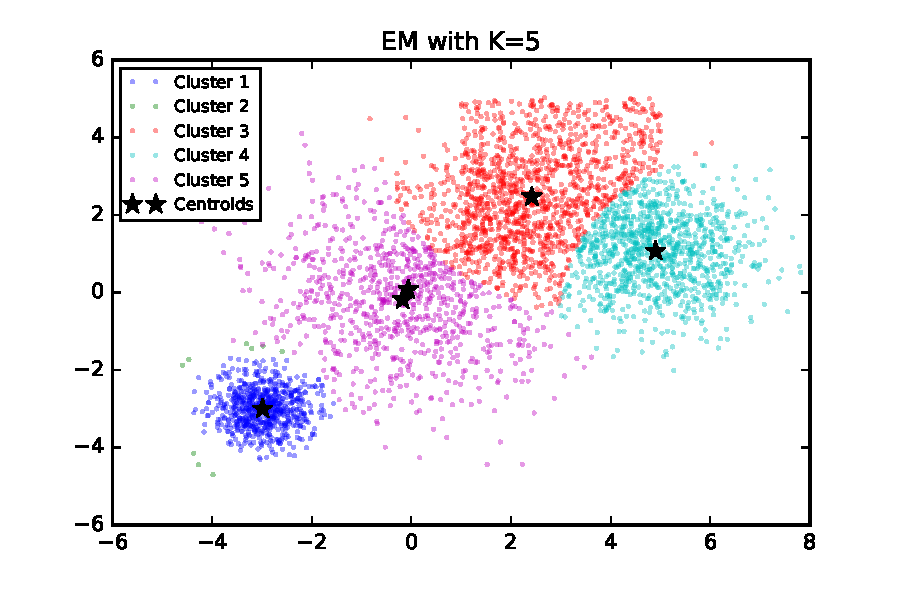
\includegraphics[width=\textwidth]{./figures/bigClustering_EM_5.pdf}
        \end{subfigure}   
        \begin{subfigure}[b]{0.475\textwidth}   
            \centering 
            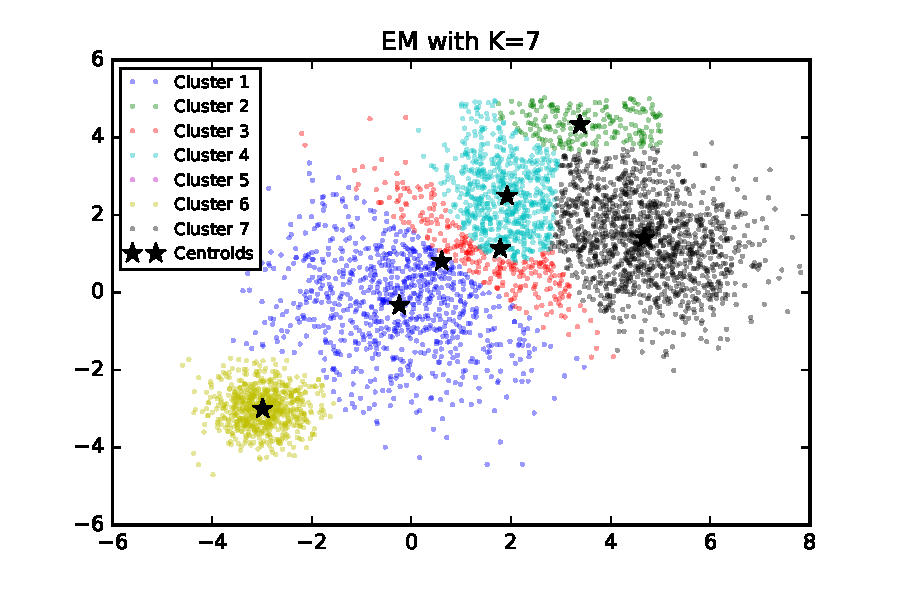
\includegraphics[width=\textwidth]{./figures/bigClustering_EM_7.pdf}
        \end{subfigure}
        \hfill
        \begin{subfigure}[b]{0.475\textwidth}   
            \centering 
            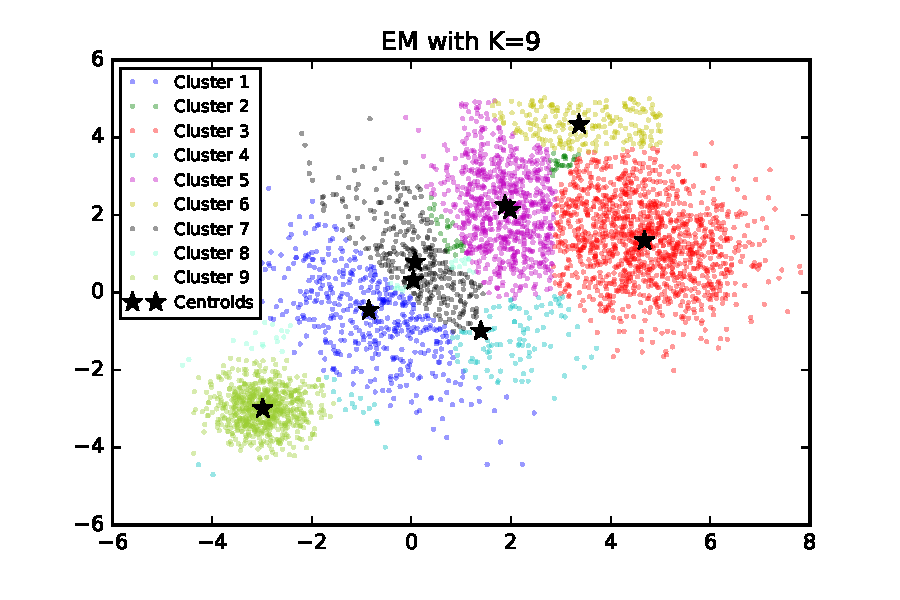
\includegraphics[width=\textwidth]{./figures/bigClustering_EM_9.pdf}
        \end{subfigure}
        
        \caption{Clustering Result for bigClusteringData.txt with EM Algorithm}
        \label{fig:EM_bigClustering}
\end{figure}

\newpage
\item{3.} The Python code used for EM Algorithm is shown in Listing 5.

% -----------------------------------------------------------------------------
\begin{lstlisting}[language=Python, caption=EM Algorithm Python Code]
import numpy as np
import time

class EM(object):
    """ self-defined calss for EM algorithm """
    def __init__(self, m, threshold=0.01, random_state=None, maxIter=500):
        """ initialize the EM algorithm """
        self.m = m
        self.threshold = threshold
        self.random_state = random_state
        self.maxIter = maxIter
        self.w = None
        self.gamma = None
        self.mu = None
        self.sigma = None
        self.gaussianProb = None
        self.logLikelihood = None
        self.distance = None
        self.D = None

    def train(self, x, verbose=False):
        """ function to perform EM algorithm on X """
        t0 = time.time()
        np.random.seed(self.random_state)

        # initialize the mean and covariance matrix
        self.initialize(x)

        # iterate through E and M steps
        for i in range(1, self.maxIter + 1):
            self.estep(x)
            self.mstep(x)
            if abs(self.logLikelihood[-1] - self.logLikelihood[-2]) \
               / abs(self.logLikelihood[-2]) < self.threshold:
                for i in range(self.m):
                    self.distance[:, i] = np.sqrt(np.sum((x - self.mu[i])**2,
                                                         axis=1))
                self.D = np.max(np.min(self.distance, axis=1))
                if verbose is True:
                    t = np.round(time.time() - t0, 4)
                    print('Reach threshold at', i,
                          'th iters in ' + str(t) + 's')
                return

        for i in range(self.m):
            self.distance[:, i] = np.sqrt(np.sum((x - self.mu[i])**2, axis=1))
        self.D = np.max(np.min(self.distance, axis=1))
        if verbose is True:
            t = np.round(time.time() - t0, 4)
            print('Stopped, reach the maximum iteration ' + str(t) + 's')

    def initialize(self, x):
        """ function to initialize the parameters """
        n, dim = x.shape  # find the dimensions
        self.distance = np.zeros((n, self.m))
        self.w = np.ones(self.m) * (1 / self.m)
        self.gamma = np.zeros((n, self.m))
        self.gaussianProb = np.zeros((n, self.m))
        self.mu = [None] * self.m
        self.sigma = [None] * self.m
        self.logLikelihood = []

        cov = np.cov(x.T)
        mean = np.mean(x, axis=0)
        for k in range(self.m):
            self.mu[k] = mean + np.random.uniform(-0.5, 0.5, dim)
            self.sigma[k] = cov

        # update gamma
        self.gamma = self.gammaprob(x, self.w, self.mu, self.sigma)

        # calculate the expectation of log-likelihood
        self.logLikelihood.append(self.likelihood())

    def estep(self, x):
        """ function to conduct E-Step for EM algorithm """
        self.gamma = self.gammaprob(x, self.w, self.mu, self.sigma)

    def mstep(self, x):
        """ function to conduct M-Step for EM algorithm """
        n, dim = x.shape
        sumGamma = np.sum(self.gamma, axis=0)
        self.w = sumGamma / n

        for k in range(self.m):
            self.mu[k] = np.sum(x.T * self.gamma[:, k], axis=1) / sumGamma[k]
            diff = x - self.mu[k]
            weightedDiff = diff.T * self.gamma[:, k]
            self.sigma[k] = np.dot(weightedDiff, diff) / sumGamma[k]
            if np.linalg.matrix_rank(self.sigma[k]) != 3:
                randv = np.random.random(dim) / 10000
                self.sigma[k] = self.sigma[k] + np.diag(randv)

        # calculate the expectation of log-likelihood
        self.logLikelihood.append(self.likelihood())

    def gammaprob(self, x, w, mu, sigma):
        """ function to calculate the gamma probability """
        for k in range(self.m):
            self.gaussianProb[:, k] = self.gaussian(x, mu[k], sigma[k])

        weightedSum = np.sum(w * self.gaussianProb, axis=1)
        gamma = ((w * self.gaussianProb).T / weightedSum).T

        return gamma

    def gaussian(self, x, mu, sigma):
        """ function to calculate the multivariate gaussian probability """
        inversion = np.linalg.inv(sigma)
        part1 = (-0.5 * np.sum(np.dot(x - mu, inversion) * (x - mu), axis=1))
        part2 = 1 / ((2 * np.pi) ** (len(mu) / 2) *
                     (np.linalg.det(sigma) ** 0.5))

        pdf = part2 * np.exp(part1)

        return pdf

    def likelihood(self):
        """ function to calculate the log likelihood """
        log = np.log(np.sum(self.w * self.gaussianProb, axis=1))
        logLikelihood = np.sum(log)

        return logLikelihood

    def get_label(self):
        """ function to predict the classes using calculated parameters """
        label = np.argmax(self.w * self.gaussianProb, axis=1)

        return label
\end{lstlisting}

% -----------------------------------------------------------------------------
\item{4.} Different Initialization Comparison.

In EM algorithm, we run 50 times with different initialization, the best result of D is shown in Table \ref{table:best_EM}.

\begin{table}[H]
	\centering
	\caption{Best Result (D) for EM Algorithm}
	\label{table:best_EM}	
	\begin{tabular}{ c | c | c | c | c | c | c | c | c | c}
		\hline \hline
		Data / K      & 2     &    3    & 4    & 5     & 6    & 7    & 8   & 9    & 10 \\[0.1cm]
		\hline
	clustering	        & 5.0744 &    4.8260 & 4.2467 & 4.1715 & 3.8116 & 3.7734 & 3.4768 & 3.4228 & 3.2690 \\[0.1cm]
bigClusteringData & N.A. &    5.4054 & 4.8813 & 4.5730 & 4.0522 & 3.8400 & 3.5024 & 3.4828 & 3.4400 \\[0.1cm]
		\hline	
	\end{tabular}
\end{table}

% -----------------------------------------------------------------------------
\item{5.} Cluster Index Comparison.

In EM algorithm, the cluster index set C (first 20) for the best result is shown in Table \ref{table:index_EM_clustering} and Table \ref{table:index_EM_bigClustering}.

\begin{table}[H]
	\centering
	\caption{Index (first 20) for EM Algorithm (clustering.txt)}
	\label{table:index_EM_clustering}	
	\begin{tabular}{ c | c }
		\hline \hline
		K        &    Index  \\[0.1cm]
		\hline
		2      & 0 0 0 0 0 0 0 0 0 0 0 0 0 0 0 0 0 0 0 0 \\[0.1cm]
		3     &  0 0 0 0 0 0 0 0 0 0 0 0 0 0 0 0 0 0 0 0 \\[0.1cm]
		4     &  0 3 3 0 1 3 3 0 1 3 1 0 1 1 0 1 1 0 3 3 \\[0.1cm]
		5     &  3 0 0 3 0 1 1 3 0 1 1 3 0 4 3 0 0 4 0 1 \\[0.1cm]
		6     &  2 0 0 0 1 2 2 5 3 2 2 2 1 3 5 2 2 3 2 2 \\[0.1cm]
		7     &  4 4 4 4 2 0 4 3 0 4 0 3 2 0 3 0 0 3 4 0 \\[0.1cm]
		8     &  6 6 5 6 5 6 6 0 6 6 6 6 3 4 0 6 6 0 6 6 \\[0.1cm]
		9     &  3 3 7 3 7 3 3 0 2 3 3 3 6 2 0 3 3 0 3 3 \\[0.1cm]
		10   &  6 6 3 6 9 8 8 6 8 6 8 3 0 8 4 8 9 7 6 8 \\[0.1cm]
		\hline	
	\end{tabular}
\end{table}

\begin{table}[H]
	\centering
	\caption{Index (first 20) for EM Algorithm (bigClusteringData.txt)}
	\label{table:index_EM_bigClustering}	
	\begin{tabular}{ c | c }
		\hline \hline
		K    & Index \\[0.1cm]
		\hline
		3     &  0 1 2 1 1 2 1 2 1 2 1 1 0 0 1 1 1 1 1 1 \\[0.1cm]
		4     &  2 1 3 0 0 3 0 3 1 3 1 0 2 2 1 0 1 1 1 0 \\[0.1cm]
		5     &  0 4 1 4 4 1 3 1 4 1 4 2 0 0 4 2 4 4 4 2 \\[0.1cm]
		6     &  2 1 3 1 1 3 5 3 1 3 1 0 2 2 1 5 4 1 4 1 \\[0.1cm]
		7     &  0 3 2 6 6 2 4 2 6 2 3 1 0 0 3 4 0 3 3 6 \\[0.1cm]
		8     &  7 5 0 2 2 0 4 0 5 0 5 6 7 7 5 4 7 5 5 2 \\[0.1cm]
		9     &  2 1 8 7 7 8 1 8 1 8 1 3 2 2 1 7 2 1 1 7 \\[0.1cm]
		10   &  4 5 1 2 2 1 9 1 5 1 5 7 4 4 5 9 8 5 5 2 \\[0.1cm]
		\hline	
	\end{tabular}
\end{table}
\end{description}

\end{description}


% -----------------------------------------------------------------------------
\section{\Large Natural Clusters Discussion}

The distribution of clustering.txt and bigClusteringData.txt are shown in Fig. \ref{fig:16a} and Fig. \ref{fig:16b}.
%  -----------------------------------------------------------------------------
\begin{figure}[H]
\centering
\centering
        \begin{subfigure}[b]{0.49\textwidth}
            \centering
            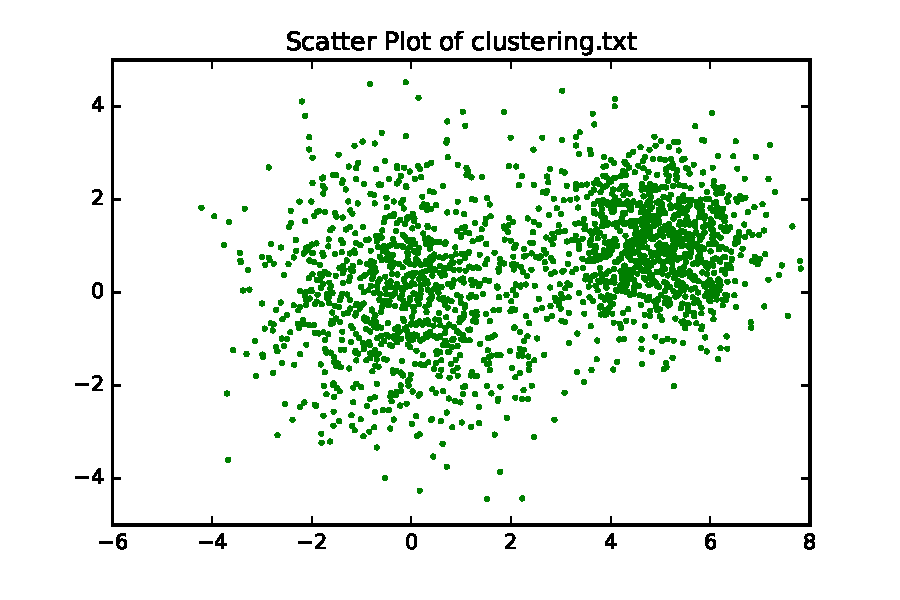
\includegraphics[width=\textwidth]{./figures/clustering_scatter.pdf}
            \caption{clustering.txt}\label{fig:16a}
        \end{subfigure}
        \hfill
        \begin{subfigure}[b]{0.49\textwidth}  
            \centering 
            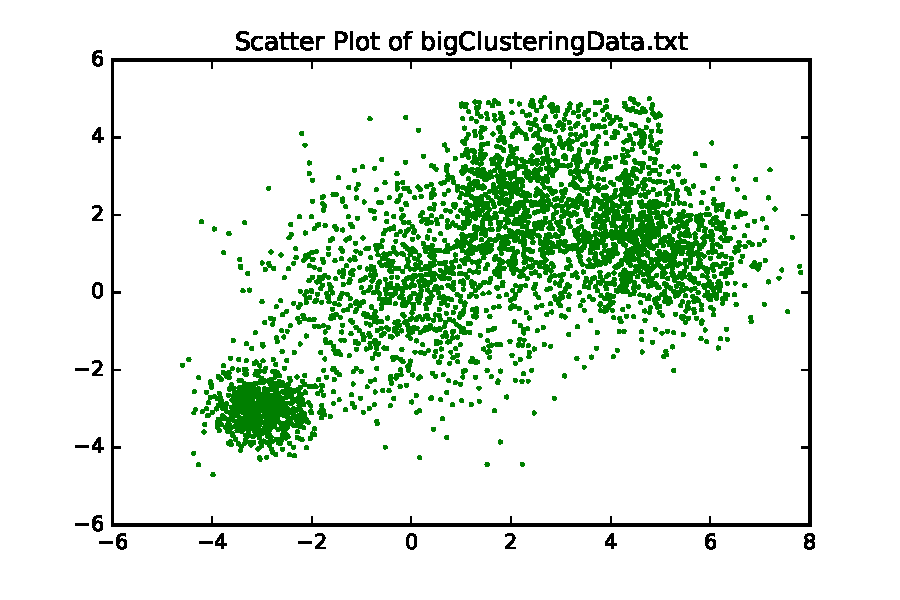
\includegraphics[width=\textwidth]{./figures/bigClustering_scatter.pdf}
            \caption{bigClusteringData.txt}\label{fig:16b}
        \end{subfigure}
\caption{Scatter Plot of Original Data}
\label{fig:clusters} 
\end{figure}

From Fig. \ref{fig:16a} and Fig. \ref{fig:16b}, the natural clusters is: 2 clusters for clustering.txt and 4 clusters for bigClusteringData.txt. This is determined by personal observation. \\

% -----------------------------------------------------------------------------
\section{\Large K-Means Convergence Discussion}

In Lloyd's algorithm, we choose 
    $$D = \underset{x_i \in X}{\max}( \underset{c_j \in Q}{\min}{||x_i - c_j||_2})$$
as the cost, the stop criterion is: 
    $$|D^{p+1} - D^{p}| < tol$$
where tol is user-defined.

Reason: as the clustered data get close to the local optimum, the cost D will decrease slower and slower. Finally, it will reach the local minimum. So, the difference between new cost and previous cost should be smaller and smaller. So, $|D^{p+1} - D^{p}| < tol$ can be used as the stop criterion.\\

% -----------------------------------------------------------------------------
\section{\Large Computational Effort Discussion}

In this part, we run those 5 algorithms on the same dataset, and report the total running time, which is shown in Table \ref{table:time_clustering} and Table \ref{table:time_bigClustering}.

\begin{table}[H]
	\centering
	\caption{Computation Time Comparison for clustering.txt}
	\label{table:time_clustering}	
	\begin{tabular}{ c | c | c | c | c | c }
		\hline \hline
		K  	&	K-Means    & K-Centers    & Single-Swap    & Spectral Clustering    & EM \\[0.1cm]
		\hline
		3	   &	0.2673     & 0.0067   & 0.1582    & 1.5716    & 0.4412 \\[0.1cm]
		4    &	0.2543     & 0.0010   & 0.1971    & 1.4587    & 0.5078 \\[0.1cm]
		5    &	0.3624     & 0.0012   & 0.1895    & 1.4132    & 0.4881 \\[0.1cm]
		6    &	0.4325     & 0.0013   & 0.2668    & 1.4840    & 0.7462 \\[0.1cm]
		7    &	0.2837     & 0.0015   & 0.2693    & 1.4877    & 0.8227 \\[0.1cm]
		8    &	0.1923     & 0.0019   & 0.3306    & 1.4708    & 0.9216 \\[0.1cm]
		9    &	0.3481     & 0.0024   & 0.3012    & 1.4669    & 1.0106 \\[0.1cm]
		10  &	0.1989     & 0.0026   & 0.3790    & 1.5053    & 1.1277 \\[0.1cm]
		\hline	
	\end{tabular}
\end{table}
{\centering Note: all measured time is in unit of seconds (s)}

\begin{table}[H]
	\centering
	\caption{Computation Time Comparison for bigClusteringData.txt}
	\label{table:time_bigClustering}	
	\begin{tabular}{ c | c | c | c | c | c }
		\hline \hline
		K  	&	K-Means     & K-Centers    & Single-Swap    & Spectral Clustering    & EM \\[0.1cm]
		\hline
		3	   &	0.4725     & 0.0020   & 0.4511    & 11.1860    & 0.3412 \\[0.1cm]
		4    &	0.8326     & 0.0019   & 0.5692    & 10.2542    & 0.2553 \\[0.1cm]
		5    &	0.4722     & 0.0021   & 0.6445    & 10.5166    & 0.5763 \\[0.1cm]
		6    &	1.2580     & 0.0024   & 0.8809    & 10.2167    & 0.6196 \\[0.1cm]
		7    &	0.9619     & 0.0025   & 0.7638    & 9.8986      & 1.1591 \\[0.1cm]
		8    &	0.7767     & 0.0034   & 0.7815    & 9.4616      & 1.3177 \\[0.1cm]
		9    &	0.7177     & 0.0037   & 0.9010    & 9.8733      & 1.4977 \\[0.1cm]
		10    &	1.2369     & 0.0041   & 1.0744    & 9.8636      & 1.7560 \\[0.1cm]
		\hline	
	\end{tabular}
\end{table}
{\centering Note: all measured time is in unit of seconds (s)}\\


From Table \ref{table:time_clustering} and Table \ref{table:time_bigClustering}, the K-Centers algorithm is the fastest and Spectral Clustering is the lowest. Fero the other algorithms, they are pretty similar. This is consistent with my analysis. For spectral clustering, since we need to compute the eigenvector, it will cost more time. For K-Centers algorithm, since we just just greedy methods to find k centers, it will be much faster. For the other method, their difference is not very clear since the dataset is not too big.

% -----------------------------------------------------------------------------
\section{\Large Single-Swap Algorithm Discussion}

The final cost for Greedy K-Centers algorithm and Single-Swap algorithm are shown in Table \ref{table:best_kcenter2} and Table \ref{table:best_single2}. With Single-Swap, the improvement of cost is clear.

\begin{table}[H]
	\centering
	\caption{Best Result (D) for K-Centers Algorithm}
	\label{table:best_kcenter2}	
	\begin{tabular}{ c | c | c | c | c | c | c | c | c | c}
		\hline \hline
		Data / K      & 2     &    3    & 4    & 5     & 6    & 7    & 8   & 9    & 10 \\[0.1cm]
		\hline
	clustering	        & 5.2838 &    4.8162 & 4.1387 & 3.7503 & 3.4691 & 3.1323 & 2.7510 & 2.7206 & 2.4634 \\[0.1cm]
bigClusteringData & N.A. &    5.5288 & 4.1446 & 3.8318 & 3.3765 & 3.2933 & 3.0093 & 2.7431 & 2.6249 \\[0.1cm]
		\hline	
	\end{tabular}
\end{table}

\begin{table}[H]
	\centering
	\caption{Best Result (D) for Single-Swap Algorithm}
	\label{table:best_single2}	
	\begin{tabular}{ c | c | c | c | c | c | c | c | c | c}
		\hline \hline
		Data / K      & 2     &    3    & 4    & 5     & 6    & 7    & 8   & 9    & 10 \\[0.1cm]
		\hline
	clustering	        & 4.6305 &    3.9619 & 3.7152 & 3.3236 & 3.0420 & 2.8479 & 2.5808 & 2.3493 & 2.3493 \\[0.1cm]
bigClusteringData & N.A. &    4.3388 & 3.8504 & 3.4619 & 3.2156 & 2.9379 & 2.8479 & 2.6053 & 2.4973 \\[0.1cm]
		\hline	
	\end{tabular}
\end{table}

To perform single-swap, we use all the points as the candidates.

In current version of Single-Swap algorithm, we use iterations to iterate all samples and all centers, this is not efficient. For better performance, for each swap, we can find the best candidate and the center that has largest radius, then we just need to swap them.

% -----------------------------------------------------------------------------
\section{\Large Summary}

In this report, we compare the performance of different algorithms, among all these five algorithms, K-Centers algorithm performs the fastest and Spectral Clustering performs the lowest. K-Means, Single-Swap and EM algorithm is between them. 

Among those five algorithms, EM algorithm performs well when the data can be modeled by GMMs. K-Means also performs well but may need a lot of different initializations. Greedy K-Centers algorithm performs the worst since it just find K centers in greedy way.

Using $D = \underset{x_i \in X}{\max}( \underset{c_j \in Q}{\min}{||x_i - c_j||_2})$ as the cost, we can find that with more clusters, $D$ will be smaller.

\clearpage

\end{document}

